% -*- mode: LaTeX; TeX-PDF-mode: t; -*- # Tell emacs the file type (for syntax)
\newcommand{\econtexRoot}{.}

\documentclass[\econtexRoot/HAFiscal]{subfiles}
\onlyinsubfile{\externaldocument{\econtexRoot/HAFiscal}} % Get xrefs -- esp to apndx -- from main file; only works if main file has already been compiled

\begin{document}

\hypertarget{introduction}{}\par\section{Introduction}\notinsubfile{\label{sec:intro}}
\setcounter{page}{0}\pagenumbering{arabic}

Fiscal policies that aim to boost consumer spending in recessions have been tried in many countries in recent decades.  The nature of such policies has varied widely, perhaps because traditional macroeconomic models have not provided plausible guidance about which ones are likely to be most effective---either in reducing misery (a `welfare metric') or in increasing output (a `GDP metric').

But a new generation of macro models has shown that when microeconomic heterogeneity across consumer circumstances (wealth; income; education) is taken into account, the consequences of an income shock for consumer spending depend on a measurable object: the intertemporal marginal propensity to consume (iMPC) introduced in \cite{auclert2018IKC}.  The iMPC extends the notion of marginal propensity to consume to account for the speed at which households spend.  Fortuitously, new sources of microeconomic data, particularly from Scandinavian national registries, have recently allowed the first high-quality measurements of the iMPC (\cite{fagereng_mpc_2021}).

Even in models that can match a given measured iMPC pattern, the relative merits of alternative policies depend profoundly both on the metric (welfare or GDP) and on the quantitative structure of the rest of the model -- for example, whether multipliers exist and whether the degree of multiplication is different under different economic conditions. Here, after constructing a microeconomically credible heterogeneous agent (HA) model, we examine that model's implications for how effects of stimulus policies depend on the existence and timing of any ``multipliers,'' which, following \cite{kmpHandbook2016}, we model in a clean and simple way, so that the interaction of the multiplier (if any) with the other elements of the model is reasonably easy to understand. %To ease interpretation of our results, as well as to keep the model tractable, our primary analysis is based on an aggregation of individual consumption responses.
This partial equilibrium analysis allows us to transparently incorporate the possibility that multipliers may be larger in recessions.  But we understand that a richer general equilibrium framework could introduce transmission channels absent from the partial-equilibrium-plus-multiplier analysis, so we also analyze a standard HANK-and-SAM general equilibrium model modified to embed our households' consumption responses.\footnote{The \href{https://econ-ark.org}{Econ-ARK} toolkit with which the partial equilibrium model was solved constructs the Jacobians necessary to connect a steady-state version of the model to the \href{https://github.com/shade-econ/sequence-jacobian}{SSJ Toolkit}. Our HANK-and-SAM model builds on \cite{Ravn2017,Ravn2021}.}

\hypertarget{microeconomically-credible}{}
By ``microeconomically credible,'' we mean a model that can match both the cross-sectional distribution of liquid wealth (following \cite{kaplan2014model}'s definition of liquid wealth) and the entire pattern of the iMPC from \cite{fagereng_mpc_2021} (see Figure~\ref{fig:aggmpclotterywin} for their data and our model's fit to it).

\hypertarget{excess-initial-mpc}{}
Standard HA models can match both the pattern of spending in years 1-4 (for a shock that arrives in year 0) and the initial distribution of liquid wealth.\footnote{For example, the model in \cite{cstwMPC}.}  But even a brief look at the figure convinces the eye that spending in the initial period when the shock arrives seems out of line with the smooth pattern of declining iMPC points in years 1-4.  The eye is not wrong: HA models that match liquid assets and the spending pattern in years 1-4 seriously underpredict the amount of immediate spending that occurs on receipt of the income shock.

We call this initial extra spending the `excess initial MPC.'  Below, we describe a substantial and longstanding literature in which the pattern of an excess initial MPC has been documented, and a vigorous recent literature confirming the fact with different datasets and proposing various potential theoretical explanations.

If multipliers are operative only in recessions (or are more powerful in recessions), a model that fails to capture the excess initial MPC might generate the wrong answers for the effectiveness of the alternative fiscal policies.

The purpose of our paper is not to weigh in on which of the alternative models of an excess initial MPC is right.  Instead we sought the simplest modeling device that would capture the empirical fact of an excess initial MPC and permit unambiguous welfare calculations.  We accomplish this by adding to the standard model something we call ``splurge'' beahavior, in which each household has a portion of income out of which they have a high MPC, and the remainder of their income is disposed of as in standard micro models with mildly impatient but time-consistent consumers.  Because the available evidence finds high initial MPCs even among wealthy households, we assume that this splurge behavior is the same across households and independent of their liquid wealth holdings.\footnote{Proponents of the theoretical models described in our literature review in section \ref{sec:lit} may choose to think of our splurge as a reduced form for a deeper explanation; we would not necessarily resist such an interpretation.}

Our resulting structural model could be used to evaluate a wide variety of consumption stimulus policies.  We examine three that have been implemented in recent recessions in the United States\ (and elsewhere): an extension of unemployment insurance (UI) benefits, a means-tested stimulus check, and a payroll tax cut.    

Our first metric of policy effectiveness is ``spending bang for the buck'': For a dollar of spending on a particular policy, how much multiplication is induced?  %Timing matters because in our model (following the empirical literature), the size of any ``consumption multiplier'' depends on the economic conditions that prevail when the extra spending occurs.  Our strategy to illuminate this point is twofold.
First, we calculate the policy-induced spending dynamics in an economy with no multiplier.  We then follow \cite{kmpHandbook2016}'s approach to modeling the aggregate demand externality, in which output depends mechanically on the level of consumption relative to steady state. But in our model, the aggregate demand externality is only switched on when the economy is experiencing a recession---there is no multiplication for spending that occurs after our simulated recession is over.  %A less stark assumption for example, the degree of multiplication depends on the distance of the economy from its steady state, or the endogenous time-varying multiplication that arises in a New-Keynesian model)would perhaps be more realistic but also much harder to assess clearly.

Because our model's outcomes reflect the behavior of utility-maximizing consumers, we can calculate another, possibly more interesting, measure of the effectiveness of alternative policies:  their effect on consumers' welfare.  Even without multiplication, a utility-based metric can justify countercyclical policy because the larger idiosyncratic shocks to income that occur during a recession may justify a greater-than-normal degree of social insurance.  We call this ``welfare bang for the buck.''

The principal difference between the two metrics is that what matters for the degree of spending multiplication is how much of the policy-induced extra spending occurs during the recession (when the multiplier matters), while effectiveness in the utility metric also depends on who is doing the extra spending (because the recession hits some households much harder than others).

Because high-MPC consumers tend to have high marginal utility, a standard aggregated welfare function would favor redistribution to such consumers even in the absence of a recession. We are interested in the degree of \textit{extra} motivation for social insurance that is present in a recession, so we construct our social welfare metric specifically to measure only the \textit{incremental} social welfare effect of alternative policies during recessions (beyond whatever redistributional logic might apply during expansions -- see section~\ref{sec:welfare}).

%Households do not prepare for our ``MIT shock'' recessions, which double the unemployment rate and the average length of unemployment spells. The end of the recession occurs as a Bernoulli process calibrated for an average recession length of six quarters, leading to a return of the unemployment rate to normal levels over time.
When the multiplier is active, any reduction in aggregate consumption below its steady-state level directly reduces aggregate productivity and thus labor income. Hence, any policy stimulating consumption will also boost incomes through this aggregate demand multiplier channel.

% We parametrize the model in two steps.  First, we estimate the extent to which consumers `splurge' when receiving an income shock. We do so using Norwegian data because it offers the best available evidence on the time profile of the marginal propensity to consume (provided by \cite{fagereng_mpc_2021}). Next we move on to the calibration of the full model on US data taking the splurge-factor as given. In the model, consumers are \textit{ex-ante} heterogeneous: The population consists of types that differ according to their level of education (which affects measured facts about permanent income and income dynamics), and their pure time-discount factors, whose distribution is estimated separately for each education group to match the liquid wealth distribution within that group. In addition, agents experience different histories of idiosyncratic income shocks and periods of unemployment, so that within each type there is \textit{ex-post} heterogeneity induced by different shock realizations. 

Our results are intuitive.  In the economy with no recession multiplier, the benefit of a sustained payroll tax cut is negligible.\footnote{One reason there is any (welfare) benefit at all, even for people who have not experienced an unemployment spell, is that the heightened risk of unemployment during a recession increases the marginal value of current income because it helps them build extra precautionary reserves to buffer against the extra risk.  A second benefit is that, for someone who becomes unemployed some time into the recession, the temporary tax reduction will have allowed them to accumulate a larger buffer to sustain them during unemployment.  Finally, in a recession, there are more people who will have experienced a spell of unemployment, and the larger population of beneficiaries means that the consequences of the prior mechanism will be greater.  But, quantitatively, all of these effects are small.}
When a multiplier exists, the tax cut has more benefits, especially if the recession continues long enough that most of the spending induced by the tax cut happens while the economy is still in recession (and the multiplier still is in force).  The typical recession, however, ends long before our `sustained' wage tax cut is reversed---and even longer before lower-MPC consumers have spent down most of their extra after-tax income. Accordingly, even in an economy with a multiplier that is powerful during recessions, much of the wage tax cut's effect on consumption occurs when any multiplier that might have existed in a recession is no longer operative.

Even leaving aside any multiplier effects, the stimulus checks improve welfare more than the wage tax cut, because at least a portion of such checks go to unemployed people who have both high MPCs and high marginal utilities (while wage tax cuts, by definition, go only to persons who are employed and earning wages). The greatest ``welfare bang for the buck'' comes from the UI insurance extension, because many of the recipients are in circumstances in which they have a much higher marginal utility than they would have had in the absence of the recession, whether or not the aggregate demand externality exists.

And, in contrast to the wage-tax cut, both the UI extension and the stimulus checks concentrate most of the marginal increment to consumption at times when the multiplier (if it exists) is still powerful.  A disadvantage of the UI extension relative to the stimulus checks, in terms of ``spending bang for the buck,'' is that it takes somewhat more time until the transfers reach the beneficiaries. The stimulus checks are assumed to be distributed immediately in the same quarter as the recession starts. Countering this disadvantage is the fact that the MPC of UI recipients is higher than that of stimulus check recipients, and, furthermore, the insurance nature of the UI payments reduces the precautionary saving motive. In the end, our model says that these two forces roughly balance each other, so that the spending bang for the buck of the two policies is similar. In the welfare metric, however, there is considerable marginal value to UI recipients even if they receive some of the benefits after the recession is over (and no multiplier exists). Hence, in the welfare metric, the relative value of UI benefits is increased compared with the policy of sending stimulus checks.

We conclude that extended UI benefits should be the first weapon employed from this arsenal, as they have a greater welfare benefit than stimulus checks and a similar (multiplied) spending effect.  But a disadvantage is that the total amount of stimulus that can be accomplished with the UI extension is constrained by the fact that only a limited number of people become unemployed.  If more stimulation is called for than can be accomplished via the UI extension, checks have the advantage that their effects scale almost linearly in the size of the stimulus---see \cite{beraja2023size} for a more detailed exposition of the relation between MPC and stimulus size.  The wage tax cut is also, in principle, scalable, but its effects are smaller because recipients have lower MPCs and marginal utility than check and UI recipients.  In the real world, a tax cut is also likely the least flexible of the three tools:  UI benefits can be further extended, and multiple rounds of checks can be sent, but multiple rounds of changes in payroll tax rates would likely be administratively and politically more difficult.

One theme of our paper is that which policies are better or worse, and by how much, depends on both the quantitative details of the policies and the quantitative modeling of the economy.  

But the tools we are using could be reasonably easily modified to evaluate a number of other policies.  For example, in the COVID-19 recession in the US, not only was the duration of UI benefits extended, but those benefits were also supplemented by substantial extra payments to every UI recipient.  We did not calibrate the model to match this particular policy, but the framework could accommodate such an analysis.


\onlyinsubfile{\bibliography{\bibfilesfound}}


%\onlyinsubfile{bibliography_blend}
%\onlyinsubfile{% Allows two (optional) supplements to hard-wired \texname.bib bibfile:
% global.bib is a default bibfile that supplies anything missing elsewhere
% Add-Refs.bib is an override bibfile that supplants anything in \texfile.bib or global.bib
\provideboolean{AddRefsExists}
\provideboolean{globalExists}
\provideboolean{BothExist}
\provideboolean{NeitherExists}
\setboolean{BothExist}{true}
\setboolean{NeitherExists}{true}

\IfFileExists{\econtexRoot/Add-Refs.bib}{
  % then
  \typeout{References in Add-Refs.bib will take precedence over those elsewhere}
  \setboolean{AddRefsExists}{true}
  \setboolean{NeitherExists}{false} % Default is true
}{
  % else
  \setboolean{AddRefsExists}{false} % No added refs exist so defaults will be used
  \setboolean{BothExist}{false}     % Default is that Add-Refs and global.bib both exist
}

% Deal with case where global.bib is found by kpsewhich
\IfFileExists{/usr/local/texlive/texmf-local/bibtex/bib/global.bib}{
  % then
  \typeout{References in default global global.bib will be used for items not found elsewhere}
  \setboolean{globalExists}{true}
  \setboolean{NeitherExists}{false}
}{
  % else
  \typeout{Found no global database file}
  \setboolean{globalExists}{false}
  \setboolean{BothExist}{false}
}

\ifthenelse{\boolean{showPageHead}}{ %then
  \clearpairofpagestyles % No header for references pages
  }{} % No head has been set to clear

\ifthenelse{\boolean{BothExist}}{
  % then use both
  \typeout{bibliography{\econtexRoot/Add-Refs,\econtexRoot/\texname,global}}
  \bibliography{\econtexRoot/Add-Refs,\econtexRoot/\texname,global}
  % else both do not exist
}{ % maybe neither does?
  \ifthenelse{\boolean{NeitherExists}}{
    \typeout{bibliography{\texname}}
    \bibliography{\texname}}{
    % no -- at least one exists
    \ifthenelse{\boolean{AddRefsExists}}{
      \typeout{bibliography{\econtexRoot/Add-Refs,\econtexRoot/\texname}}
      \bibliography{\econtexRoot/Add-Refs,\econtexRoot/\texname}}{
      \typeout{bibliography{\econtexRoot/\texname,global}}
      \bibliography{        \econtexRoot/\texname,global}}
  } % end of picking the one that exists
} % end of testing whether neither exists
}

\ifthenelse{\boolean{Web}}{}{
%  \onlyinsubfile{\captionsetup[figure]{list=no}}
%  \onlyinsubfile{\captionsetup[table]{list=no}}
  \end{document} \endinput
}

\endinput

\hypertarget{related-literature}{}\par\subsection{Related literature}
\notinsubfile{\label{sec:lit}}

Several papers have looked at fiscal policies that have been implemented in the U.S.\ through the lens of a structural model. \cite{coenen2012effects} analyses the effects of different fiscal policies using seven different models. The models are variants of two-agent heterogeneous agent models and make no attempt to match the full distribution of liquid wealth as we do in this paper. We also attempt to match the microdata on household consumption behavior, much of which has come more recently.  More closely aligned to the methodology of our paper are \cite{mckay2016role}, \cite{mckay2021optimal}, and \cite{phan2024welfare} which look at the role of automatic stabilizers. By contrast, we consider discretionary policies that have been invoked after a recession has begun. Another related paper is \cite{bayercoronavirus} who studies fiscal policies implemented during the pandemic. They find that targeted stimulus through an increase in unemployment benefits has a much larger multiplier than an untargeted policy. In contrast, we find that untargeted stimulus checks have slightly higher multiplier effects when compared with a targeted policy extending eligibility for unemployment insurance. Our results derive from the fact that---as in the data---even high liquid wealth consumers have relatively high MPCs in our model.

This paper is also closely related to the empirical literature that aims to estimate the effect of transitory income shocks and stimulus payments. We particularly focus on \cite{fagereng_mpc_2021}, who use Norwegian administrative panel data with sizable lottery wins to estimate the MPC out of transitory income in that year, as well as the pattern of expenditure in the following years. We build a model that is consistent with the patterns they identify. Examples of the literature that followed the Great Recession in 2008 are \cite{parker2013consumer} and \cite{broda2014economic}. These papers exploit the effectively random timing of the distribution of stimulus payments and identify a substantial consumption response. The results indicate an MPC that is difficult to reconcile with representative agent models.

Thus, the paper relates to the literature presenting HA models that aim to be consistent with the evidence from the micro-data. An example is \cite{kaplan2014model}, who build a model where agents save in both liquid and illiquid assets. The model yields a substantial consumption response to a stimulus payment, since MPCs are high both for constrained, low-wealth households and for households with substantial net worth that is mainly invested in the illiquid asset (the ``wealthy hand-to-mouth''). \cite{carroll2020modeling} present an HA model that is similar in many respects to the one we study. Their focus is on predicting the consumption response to the 2020 U.S.\ CARES Act that contains both an extension of unemployment benefits and a stimulus check. However, neither of these papers attempts to evaluate and rank the effectiveness of different stimulus policies, as we do.

\cite{kaplanMPC2022} discuss different mechanisms used in HA models to obtain a high MPC and the tension between that and fitting the distribution of aggregate wealth. We use one of the mechanisms they consider, \textit{ex-ante} heterogeneity in discount factors, and build a model that delivers both high average MPCs and a distribution of liquid wealth consistent with the data. The model allows for splurge consumption and thus also delivers substantial MPCs for high-liquid-wealth households. This helps the model match not only the initial MPC, but also the propensity to spend out of a windfall for several periods after it is obtained.

In our model, consumers do not adjust their labor supply in response to the stimulus policies.  Our assumption is broadly consistent with the empirical findings in \cite{ganong2022spending} and \cite{chodorow2016limited}. However, the literature is conflicted on this subject and \cite{hagedorn2017impact} and \cite{hagedorn2019unemployment} find that extensions of unemployment insurance affect both search decisions and vacancy creation leading to a rise in unemployment. \cite{kekre2022unemp}, on the other hand, evaluates the effect of extending unemployment insurance in the period from 2008 to 2014. He finds that this extension raised aggregate demand and implied a lower unemployment rate than without the policy. However, he does not attempt to compare the stimulus effects of extending unemployment insurance with other policies.

One criterion to rank policies is the extent to which spending is ``multiplied,'' and our paper therefore relates to the vast literature discussing the size and timing of any multiplier. Our focus is on policies implemented in the aftermath of the Great Recession, a period when monetary policy was essentially fixed at the zero lower bound (ZLB). We therefore do not consider monetary policy responses to the policies we evaluate in our primary analysis, and our work thus relates to papers such as \cite{christiano2011government} and \cite{eggertsson2011fiscal}, who argue that fiscal multipliers are higher in such circumstances. \cite{hagedorn2019fiscal} present an HA model with both incomplete markets and nominal rigidities to evaluate the size of the fiscal multiplier and also find that it is higher when monetary policy is constrained. Unlike us, they focus on government spending instead of transfers and are interested in different options for financing that spending. \cite{broer2023fiscalmultipliers} also focus on fiscal multipliers for government spending and show how they differ in representative agent and HA models with different sources of nominal rigidities. \cite{ramey2018government} investigate empirically whether there is support for the model-based results that fiscal multipliers are higher in certain states. While they find evidence that multipliers are higher when there is slack in the economy or the ZLB binds, the multipliers they find are still below one in most specifications. In any case, we condition on policies being implemented in a recession---when, this literature argues, multipliers are higher---but it is not crucial for our purposes whether the multipliers are greater than one or not. We are concerned with relative multipliers, and the multiplier is only one of the two criteria we use to rank policies. 

The second criterion to rank policies is our measure of welfare. Thus, the paper relates to the recent literature on welfare comparisons in HA models. Both \cite{bhandari2021efficiency} and \cite{davila2022welfare} introduce ways of decomposing welfare effects. In the former case, these are aggregate efficiency, redistribution and insurance, while the latter further decomposes the insurance part into intra- and intertemporal components. These papers are related to ours, but we do not decompose the welfare effects. Regardless of decomposition, we want to (1) use a welfare measure as an additional way of ranking policies and (2) introduce a measure that abstracts from any incentive for a planner to redistribute in the steady state (or ``normal'' times).

\hypertarget{organization}{}\par\subsection{Organization}
\notinsubfile{\label{sec:org}}

The paper is organized as follows. Section~\ref{sec:model} presents our baseline partial equilibrium model of households' consumption and saving problem as well as how we model a recession and the potential response in terms of three different consumption stimulus policies. Section~\ref{sec:parameters} describes the steps we take to parameterize the model and discusses the implications for some moments that we do not target. In section~\ref{sec:comparing} we compare the three policies implemented in a recession both in terms of their multipliers and in terms of a welfare measure that we introduce. Section~\ref{sec:hank} presents a general equilibrium HANK and SAM model where we compare the multipliers of the same three policies to the partial equilibrium results. Section~\ref{sec:conclusion} concludes, and, finally, the appendix shows results from a version of the model without splurge consumption and provides more details of the HANK and SAM model discussed in Section~\ref{sec:hank}. 


\onlyinsubfile{\bibliography{\bibfilesfound}}


%\onlyinsubfile{bibliography_blend}
%\onlyinsubfile{% Allows two (optional) supplements to hard-wired \texname.bib bibfile:
% global.bib is a default bibfile that supplies anything missing elsewhere
% Add-Refs.bib is an override bibfile that supplants anything in \texfile.bib or global.bib
\provideboolean{AddRefsExists}
\provideboolean{globalExists}
\provideboolean{BothExist}
\provideboolean{NeitherExists}
\setboolean{BothExist}{true}
\setboolean{NeitherExists}{true}

\IfFileExists{\econtexRoot/Add-Refs.bib}{
  % then
  \typeout{References in Add-Refs.bib will take precedence over those elsewhere}
  \setboolean{AddRefsExists}{true}
  \setboolean{NeitherExists}{false} % Default is true
}{
  % else
  \setboolean{AddRefsExists}{false} % No added refs exist so defaults will be used
  \setboolean{BothExist}{false}     % Default is that Add-Refs and global.bib both exist
}

% Deal with case where global.bib is found by kpsewhich
\IfFileExists{/usr/local/texlive/texmf-local/bibtex/bib/global.bib}{
  % then
  \typeout{References in default global global.bib will be used for items not found elsewhere}
  \setboolean{globalExists}{true}
  \setboolean{NeitherExists}{false}
}{
  % else
  \typeout{Found no global database file}
  \setboolean{globalExists}{false}
  \setboolean{BothExist}{false}
}

\ifthenelse{\boolean{showPageHead}}{ %then
  \clearpairofpagestyles % No header for references pages
  }{} % No head has been set to clear

\ifthenelse{\boolean{BothExist}}{
  % then use both
  \typeout{bibliography{\econtexRoot/Add-Refs,\econtexRoot/\texname,global}}
  \bibliography{\econtexRoot/Add-Refs,\econtexRoot/\texname,global}
  % else both do not exist
}{ % maybe neither does?
  \ifthenelse{\boolean{NeitherExists}}{
    \typeout{bibliography{\texname}}
    \bibliography{\texname}}{
    % no -- at least one exists
    \ifthenelse{\boolean{AddRefsExists}}{
      \typeout{bibliography{\econtexRoot/Add-Refs,\econtexRoot/\texname}}
      \bibliography{\econtexRoot/Add-Refs,\econtexRoot/\texname}}{
      \typeout{bibliography{\econtexRoot/\texname,global}}
      \bibliography{        \econtexRoot/\texname,global}}
  } % end of picking the one that exists
} % end of testing whether neither exists
}

\ifthenelse{\boolean{Web}}{}{
%  \onlyinsubfile{\captionsetup[figure]{list=no}}
%  \onlyinsubfile{\captionsetup[table]{list=no}}
  \end{document} \endinput
}

% -*- mode: LaTeX; TeX-PDF-mode: t; -*- # Tell emacs the file type (for syntax)
\newcommand{\econtexRoot}{.}

\documentclass[\econtexRoot/HAFiscal]{subfiles}
\onlyinsubfile{\externaldocument{\econtexRoot/HAFiscal}} % Get xrefs -- esp to apndx -- from main file; only works if main file has already been compiled

\begin{document}

\hypertarget{related-literature}{}\par\subsection{Related literature}
\notinsubfile{\label{sec:lit}}

%% HT: I've put this stuff at the top not because I think it belongs at the top
%% but to make it easy for you to find so you can relocate it as you see fit
\hypertarget{excess-initial-mpc-literature}{}
\hypertarget{kotsogiannisMPCs}{}

The evidence for an excess initial MPC in \cite{fagereng_mpc_2021} is consistent with longstanding as well as recent findings in the literature.  Perhaps the closest direct comparison is to \cite{kotsogiannisMPCs}, who use data from a Greek (as opposed to Norwegian) lottery, and find that the induced extra monthly spending in the first three months is triple the induced extra spending in the remaining observed months.\footnote{The paper also interestingly finds a close connection between reported preferences (what consumers \textit{say} they will do in a hypothetical scenario) and their actual behavior when the scenario is realized.  Other recent papers using hypothetical questions such as \cite{jappelliIntertemporal} or \cite{colarietiHow} find estimates ranging from 15 to 26 percent in the first year depending on the size of windfall gains. This suggests that it might be to fruitful to ask respondents \textit{why} they expect to exhibit a high initial MPC.}  

Because they are focused primarily on measuring empirical facts, neither of these papers proposes a specific model for the excess initial MPC (nor do most earlier papers, such as \cite{parker2013consumer,jpsTax}).  But a substantial literature has recently developed that both provides further evidence of an excess initial MPC and proposes a number of competing theoretical models of the phenomenon.  

\hypertarget{laibson2022simple}{}

One strand of the theoretical literature explores the possibility that the burst of initial spending is rationalizable if the spending is on durables  (\cite{bcShocksStocks}).  \cite{mankiw:durgoods} showed that in the frictionless case, spending on durable goods should be vastly more responsive to a permanent income shock than spending on nondurables.\footnote{Much \textit{more} responsive than the aggregate data indicate.  \cite{caballeroDurable} proposed that a heterogeneous agent model might explain the `slow adjustment,' but \cite{cdSs} have argued that when uncertainty is added to the problem, durable goods expenditures again become much more volatile than in the data.}$^{,}$\footnote{The NIPA accounts treat as `durable' those goods whose expected lifetime is 3 years or more, but at the annual frequency many more things are arguably durable -- for example, \cite{hkpMemorable} argue that many services are durable at the annual frequency, which explains why people take vacations once a year.}  It seems plausible that a model in which consumers own a large number of goods that are durable at, say, the quarterly or annual frequency\footnote{\cite{bdTimeSeriesC} mention clothes and shoes as examples.} could explain the `excess initial MPC' as actually reflecting a rational marginal propensity to Expend (MPX).  

% Summary of papers: delete later
%\cite{BoutrosWindfall}: costly re-optimization of infinite horizon consumption paths. Small windfall gains will result in less consumption-smoothing

%\cite{ilutEconomic}: Bounded rationality model of imperfect reasoning in which households keep their old policy functions until a big enough shock hits. Therefore, even unconstraint (wealthier) households have high initial MPCs.

%\cite{Lian2023-ca}: Mistakes in future consumption results in high current MPCs. Various behavioral biases can cause these mistakes, such as inattention, present bias, diagnostic expectations, and near-rationality (epsilon-mistakes).

\hypertarget{indarte2024explains}{}

Alternatively, \cite{Lian2023-ca} shows in an intertemporal consumption saving model how deviations of the optimal consumption policy in the future result in high MPCs today. These \textit{mistakes} can arise due to many behavioral biases. \cite{BoutrosWindfall} and \cite{ilutEconomic} use costly re-optimization in a model with bounded rationality, whereas \cite{indarte2024explains} and \cite{lmmPresentBias} attribute the excess initial MPX to a form of ``present bias'' in which people have strongly time inconsistent preferences.

\cite{laibson2022simple} combine these two ideas in a simple model with both present bias and durables expenditures.  A back-of-the-envelope calculation yields a rough estimate that the ratio of initial spending on durables to the spending that would occur if all spending were nondurable is roughly 3.2 to one (not far from the ratio estimated in the Greek lottery episode studied by \cite{kotsogiannisMPCs}).

A potential challenge to these interpretations is the now-substantial literature showing that even high-wealth households seem to have a high initial MPC out of income shocks.\footnote{In addition to \cite{fagereng_mpc_2021}, \cite{boehm2025fivefacts}, \cite{graham2024mental}, \cite{crawley2023MicroMacro}, and \cite{kueng2018excess} among others all provide strong evidence of high MPCs for high-liquid-wealth households.}  If such households achieved their high wealth because they are less present-biased than others, present-bias may not be a good explanation for their high MPCs; and it also seems likely to be difficult to explain why high-liquid-wealth households would have a high propensity to buy durables out of a (relatively) small transitory shock.

For our purposes, a further attraction to the idea that the initial excess MP[C/X] reflects durables expenditures is that the \cite{mankiw:durgoods} model implies that the marginal value of an extra dollar of expenditures on durables is equal to the marginal utility of an extra unit of nondurables spending. At least to first order, this justifies our choice in the welfare analysis to assume that the marginal utility of splurge spending is equal to the marginal utility of nondurables consumption.  Complications like convex adjustment costs can break this exact equality, but even in that case it seems likely that a variant of the arguments of \cite{akerlof1985near} and \cite{cochrane1989sensitivity} would hold: Small deviations of actual behavior from the behavior in an idealized model are likely to have small consequences for utility.

Several papers have looked at fiscal policies that have been implemented in the U.S.\ under the lens of a structural model. \cite{coenen2012effects} analyses the effects of different fiscal policies using seven different models. The models are variants of two-agent heterogeneous agent models and make no attempt to match the full distribution of liquid wealth as we do in this paper. We also attempt to match the microdata on household consumption behavior, much of which has come more recently.  More closely aligned to the methodology of our paper are \cite{mckay2016role}, \cite{mckay2021optimal}, and \cite{phan2024welfare} which look at the role of automatic stabilizers. By contrast, we consider discretionary policies that have been invoked after a recession has begun. Another related paper is \cite{bayercoronavirus} who studies fiscal policies implemented during the pa  ndemic. They find that targeted stimulus through an increase in unemployment benefits has a much larger multiplier than an untargeted policy. In contrast, we find that untargeted stimulus checks have slightly higher multiplier effects when compared with a targeted policy extending eligibility for unemployment insurance. Our results derive from the fact that---as in the data---even high liquid wealth consumers have relatively high MPCs in our model.

This paper is also closely related to the empirical literature that aims to estimate the effect of transitory income shocks and stimulus payments. We particularly focus on \cite{fagereng_mpc_2021}, who use Norwegian administrative panel data with sizable lottery wins to estimate the MPC out of transitory income in that year, as well as the pattern of expenditure in the following years. We build a model that is consistent with the patterns they identify. Examples of the literature that followed the Great Recession in 2008 are \cite{parker2013consumer} and \cite{broda2014economic}. These papers exploit the effectively random timing of the distribution of stimulus payments and identify a substantial consumption response. The results indicate an MPC that is difficult to reconcile with representative agent models.

Thus, the paper relates to the literature presenting HA models that aim to be consistent with the evidence from the micro-data. An example is \cite{kaplan2014model}, who build a model where agents save in both liquid and illiquid assets. The model yields a substantial consumption response to a stimulus payment, since MPCs are high both for constrained, low-wealth households and for households with substantial net worth that is mainly invested in the illiquid asset (the ``wealthy hand-to-mouth''). \cite{carroll2020modeling} present an HA model that is similar in many respects to the one we study. Their focus is on predicting the consumption response to the 2020 U.S.\ CARES Act that contains both an extension of unemployment benefits and a stimulus check. However, neither of these papers attempts to evaluate and rank the effectiveness of different stimulus policies, as we do.

\cite{kaplanMPC2022} discuss different mechanisms used in HA models to obtain a high MPC and the tension between that and fitting the distribution of aggregate wealth. We use one of the mechanisms they consider, \textit{ex-ante} heterogeneity in discount factors, and build a model that delivers both high average MPCs and a distribution of liquid wealth consistent with the data. The model allows for splurge consumption and thus also delivers substantial MPCs for high-liquid-wealth households.\footnote{In addition to \cite{fagereng_mpc_2021}, \cite{graham2024mental}, \cite{crawley2023MicroMacro}, and \cite{kueng2018excess} among others all provide strong evidence of high MPCs for high-liquid-wealth households. By contrast, the ``infrequent consumption good'' by \citet{melcangiStock} aims at accounting for high saving rates among high-income households during normal times and high consumption during episodes where the infrequent consumption good becomes available (such as high-end health care, education expenses or bequests). The high consumption is thus not triggered by a transitory income shock but by rare consumption opportunities.} This helps the model match not only the initial MPC, but also the propensity to spend out of a windfall for several periods after it is obtained.

We include splurge consumption as a model device that lets the model match the empirical evidence, but in the literature there are several attempts at explaining such behavior. One possibility is that the burst of initial spending is rationalizable if the spending is on durables \citep{bcShocksStocks}.  \cite{mankiw:durgoods} showed that in the frictionless case, spending on durable goods should be vastly more responsive to a permanent income shock than spending on nondurables. It seems plausible that a model with a large number of goods that are durable at, say, the quarterly or annual frequency could explain the `excess initial MPC' as actually reflecting a rational marginal propensity to Expend (MPX).\footnote{The NIPA accounts treat as `durable' those goods whose expected lifetime is 3 years or more, but at the annual frequency many more things are arguably durable -- for example, \cite{bdTimeSeriesC} mention clothes and shoes, and \cite{hkpMemorable} argue that many services are durable at the annual frequency, which explains why people take vacations once a year.} Alternatively, \cite{indarte2024explains} attribute the excess initial MPX to a form of ``present bias'' in which people have strongly time inconsistent preferences; \cite{lmmPresentBias} offer a similar interpretation. 

\cite{laibson2022simple} combine these two ideas in a simple model with both present bias and durables expenditures.  A back-of-the-envelope calculation yields a rough estimate that the ratio of initial spending on durables to the spending that would occur if all spending were nondurable is roughly three to one (not far from the ratio estimated in the Greek lottery episode studied by \cite{kotsogiannisMPCs}).

In our model, consumers do not adjust their labor supply in response to the stimulus policies.  Our assumption is broadly consistent with the empirical findings in \cite{ganong2022spending} and \cite{chodorow2016limited}. However, the literature is conflicted on this subject and \cite{hagedorn2017impact} and \cite{hagedorn2019unemployment} find that extensions of unemployment insurance affect both search decisions and vacancy creation leading to a rise in unemployment. \cite{kekre2022unemp}, on the other hand, evaluates the effect of extending unemployment insurance in the period from 2008 to 2014. He finds that this extension raised aggregate demand and implied a lower unemployment rate than without the policy. However, he does not attempt to compare the stimulus effects of extending unemployment insurance with other policies. Finally, \cite{cohenDisemployment} employ a meta-analysis of the literature on how unemployment benefits impact unemployment duration, and they find that the effects are modest. 

One criterion to rank policies is the extent to which spending is ``multiplied,'' and our paper therefore relates to the vast literature discussing the size and timing of any multiplier. Our focus is on policies implemented in the aftermath of the Great Recession, a period when monetary policy was essentially fixed at the zero lower bound (ZLB). We therefore do not consider monetary policy responses to the policies we evaluate in our primary analysis, and our work thus relates to papers such as \cite{christiano2011government} and \cite{eggertsson2011fiscal}, who argue that fiscal multipliers are higher in such circumstances. \cite{hagedorn2019fiscal} present an HA model with both incomplete markets and nominal rigidities to evaluate the size of the fiscal multiplier and also find that it is higher when monetary policy is constrained. Unlike us, they focus on government spending instead of transfers and are interested in different options for financing that spending. \cite{broer2023fiscalmultipliers} also focus on fiscal multipliers for government spending and show how they differ in representative agent and HA models with different sources of nominal rigidities. \cite{ramey2018government} investigate empirically whether there is support for the model-based results that fiscal multipliers are higher in certain states. While they find evidence that multipliers are higher when there is slack in the economy or the ZLB binds, the multipliers they find are still below one in most specifications. In any case, we condition on policies being implemented in a recession---when, this literature argues, multipliers are higher---but it is not crucial for our purposes whether the multipliers are greater than one or not. We are concerned with relative multipliers, and the multiplier is only one of the two criteria we use to rank policies. 

The second criterion to rank policies is our measure of welfare. Thus, the paper relates to the recent literature on welfare comparisons in HA models. Both \cite{bhandari2021efficiency} and \cite{davila2022welfare} introduce ways of decomposing welfare effects. In the former case, these are aggregate efficiency, redistribution and insurance, while the latter further decomposes the insurance part into intra- and intertemporal components. These papers are related to ours, but we do not decompose the welfare effects. Regardless of decomposition, we want to (1) use a welfare measure as an additional way of ranking policies and (2) introduce a measure that abstracts from any incentive for a planner to redistribute in the steady state (or ``normal'' times).

\hypertarget{organization}{}\par\subsection{Organization}
\notinsubfile{\label{sec:org}}

The paper is organized as follows. Section~\ref{sec:model} presents our baseline partial equilibrium model of households' consumption and saving problem as well as how we model a recession and the potential response in terms of three different consumption stimulus policies. Section~\ref{sec:parameters} describes the steps we take to parameterize the model and discusses the implications for some moments that we do not target. In section~\ref{sec:comparing} we compare the three policies implemented in a recession both in terms of their multipliers and in terms of a welfare measure that we introduce. Section~\ref{sec:hank} presents a general equilibrium HANK and SAM model where we compare the multipliers of the same three policies to the partial equilibrium results. Section~\ref{sec:conclusion} concludes, and, finally, the appendix shows results from a version of the model without splurge consumption and provides more details of the HANK and SAM model discussed in Section~\ref{sec:hank}. 


\onlyinsubfile{\bibliography{\bibfilesfound}}


%\onlyinsubfile{bibliography_blend}
%\onlyinsubfile{% Allows two (optional) supplements to hard-wired \texname.bib bibfile:
% global.bib is a default bibfile that supplies anything missing elsewhere
% Add-Refs.bib is an override bibfile that supplants anything in \texfile.bib or global.bib
\provideboolean{AddRefsExists}
\provideboolean{globalExists}
\provideboolean{BothExist}
\provideboolean{NeitherExists}
\setboolean{BothExist}{true}
\setboolean{NeitherExists}{true}

\IfFileExists{\econtexRoot/Add-Refs.bib}{
  % then
  \typeout{References in Add-Refs.bib will take precedence over those elsewhere}
  \setboolean{AddRefsExists}{true}
  \setboolean{NeitherExists}{false} % Default is true
}{
  % else
  \setboolean{AddRefsExists}{false} % No added refs exist so defaults will be used
  \setboolean{BothExist}{false}     % Default is that Add-Refs and global.bib both exist
}

% Deal with case where global.bib is found by kpsewhich
\IfFileExists{/usr/local/texlive/texmf-local/bibtex/bib/global.bib}{
  % then
  \typeout{References in default global global.bib will be used for items not found elsewhere}
  \setboolean{globalExists}{true}
  \setboolean{NeitherExists}{false}
}{
  % else
  \typeout{Found no global database file}
  \setboolean{globalExists}{false}
  \setboolean{BothExist}{false}
}

\ifthenelse{\boolean{showPageHead}}{ %then
  \clearpairofpagestyles % No header for references pages
  }{} % No head has been set to clear

\ifthenelse{\boolean{BothExist}}{
  % then use both
  \typeout{bibliography{\econtexRoot/Add-Refs,\econtexRoot/\texname,global}}
  \bibliography{\econtexRoot/Add-Refs,\econtexRoot/\texname,global}
  % else both do not exist
}{ % maybe neither does?
  \ifthenelse{\boolean{NeitherExists}}{
    \typeout{bibliography{\texname}}
    \bibliography{\texname}}{
    % no -- at least one exists
    \ifthenelse{\boolean{AddRefsExists}}{
      \typeout{bibliography{\econtexRoot/Add-Refs,\econtexRoot/\texname}}
      \bibliography{\econtexRoot/Add-Refs,\econtexRoot/\texname}}{
      \typeout{bibliography{\econtexRoot/\texname,global}}
      \bibliography{        \econtexRoot/\texname,global}}
  } % end of picking the one that exists
} % end of testing whether neither exists
}

\ifthenelse{\boolean{Web}}{}{
%  \onlyinsubfile{\captionsetup[figure]{list=no}}
%  \onlyinsubfile{\captionsetup[table]{list=no}}
  \end{document} \endinput
}

% allow latex to find custom stuff
% Add the listed directories to the search path
% (allows easy moving of files around later)
% these paths are searched AFTER local config kpsewhich

% *.sty, *.cls
\makeatletter
\def\input@path{{@resources/texlive/texmf-local/tex/latex//}
        ,{@resources/texlive/latex//}
        ,{@local//}
        }
\makeatother
\makeatletter
\def\bibinput@path{{@resources/texlive/texmf-local/tex/latex//}
        ,{@resources/texlive/latex//},
        ,{@local//}
        }
\makeatother
  

% Set paths (like, \LaTeXInputs) to find resources
\newcommand{\econtexRoot}{.}
 

\documentclass[\econtexRoot/HAFiscal]{subfiles}
\onlyinsubfile{\externaldocument{\econtexRoot/HAFiscal}} % Get xrefs -- esp to apndx -- from main file; only works if main file has already been compiled

\begin{document}
\notinsubfile{\renewcommand{\econtexRoot}{.}}

\hypertarget{model}{}\par\section{Model}
\notinsubfile{\label{sec:model}}

Consumers differ by their level of education and, within education group, by subjective discount factors (calibrated to match the within-group distribution of liquid wealth). We first describe each kind of consumer's problem, given an income process with permanent and transitory shocks calibrated to their type, as well as type-specific shocks to employment. The next step describes the arrival of a recession and the policies we study as potential fiscal policy responses. The last section discusses an extension incorporating aggregate demand effects that induce feedback from aggregate consumption to income and (via the marginal propensity to consume) back to consumption, amplifying the effect of a recession when it occurs. 

A consumer $i$ has education $e(i)$ and a subjective discount factor $\beta_i$. The consumer faces a stochastic income stream, $\mathbf{y}_{i,t}$, and chooses to consume a fraction of that income when it arrives---the `splurge', described in the introduction.\footnote{One attractive feature of the splurge assumption is that it is also consistent with evidence from \cite{ganongConsumer2019}, that spending drops sharply following the large and predictable drop in income after the exhaustion of unemployment benefits; see below.} With what is left over, the consumer chooses to optimize consumption without regard to the fraction that was already spent. Therefore, consumption each period for consumer $i$ can be written as
\begin{verbatimwrite}{\EqDir/splurge}
\begin{equation}\begin{gathered}\begin{aligned}
  \mathbf{c}_{i,t} &= \mathbf{c}_{sp,i,t} + \mathbf{c}_{opt,i,t}, \label{eq:model}
\end{aligned}\end{gathered}\end{equation}
\end{verbatimwrite}
\begin{equation}\begin{gathered}\begin{aligned}
  \mathbf{c}_{i,t} &= \mathbf{c}_{sp,i,t} + \mathbf{c}_{opt,i,t}, \label{eq:model}
\end{aligned}\end{gathered}\end{equation}

where $\mathbf{c}_{i,t}$ is total consumption, $\mathbf{c}_{sp,i,t}$ is the splurge consumption, and $\mathbf{c}_{opt,i,t}$ is the consumer's optimal choice of consumption after splurging.
Splurge consumption is simply a fraction of income:
\begin{equation}\begin{gathered}\begin{aligned}
  \mathbf{c}_{sp,i,t} = \varsigma \mathbf{y}_{i,t},
\end{aligned}\end{gathered}\end{equation}
while the optimized portion of consumption is chosen to maximize the perpetual-youth lifetime expected-utility-maximizing consumption, where $D$ is the end-of-life probability:
\begin{equation}\begin{gathered}\begin{aligned}
  \sum_{t=0}^{\infty}\beta_i^t (1-D)^t \mathbb{E}_0 u(\mathbf{c}_{opt,i,t}).
\end{aligned}\end{gathered}\end{equation}
We use a standard CRRA (constant relative risk aversion) utility function, so $u(c) = c^{1-\gamma}/(1-\gamma)$ for $\gamma \neq 1$ and $u(c) = \log(c)$ for $\gamma=1$, where $\gamma$ is the coefficient of relative risk aversion.
The optimization is subject to the budget constraint, given existing market resources $\mathbf{m}_{i,t}$ and income state, and a no-borrowing constraint: 
\begin{equation}\begin{gathered}\begin{aligned}
  \mathbf{a}_{i,t} &= \mathbf{m}_{i,t} - \mathbf{c}_{i,t}, \\ 
  \mathbf{m}_{i,t+1} &= R \mathbf{a}_{i,t} + \mathbf{y}_{i,t+1}, \\
  \mathbf{a}_{i,t} &\geq 0,  
\end{aligned}\end{gathered}\end{equation}
where $R$ is the gross interest factor for accumulated assets $\mathbf{a}_{i,t}$.

\hypertarget{the-income-process}{}\par\subsection{The income process}

Consumers face a stochastic income process with permanent and transitory shocks to income, along with unemployment shocks.
In normal times, consumers who become unemployed receive unemployment benefits for two quarters.
Permanent income evolves according to:
\begin{equation}\begin{gathered}\begin{aligned}
  \mathbf{p}_{i,t+1} = \psi_{i,t+1}\Gamma_{e(i)}\mathbf{p}_{i,t},
\end{aligned}\end{gathered}\end{equation}
where $\psi_{i,t+1}$ is the shock to permanent income and $\Gamma_{e(i)}$ is the average growth rate of income for the consumer's education group $e(i)$.\footnote{We model the rate of growth for permanent income for each education group and keep this rate unchanged during periods of unemployment.
There is evidence, e.g.\ in \cite{davis_recessions_2011}, that unemployment, especially in a recession, leads to permanent income loss.
This finding could be added to the model---see \citet{carroll2020modeling} for an example---but is not material to the evaluation of stimulus payments here so we have chosen to keep the model simple.
} The realized growth rate of permanent income for consumer $i$ is thus $\hat{\Gamma}_{i,t+1} = \psi_{i,t+1} \Gamma_{e(i)}$.
The shock to permanent income is normally distributed with variance $\sigma_{\psi}^2$.

The actual income a consumer receives will be subject to the individual's employment status as well as transitory shocks, $\xi_{i,t}$:
\begin{equation}\begin{gathered}\begin{aligned}
  \mathbf{y}_{i,t} =   \begin{cases}
    \xi_{i,t}\mathbf{p}_{i,t}, & \text{if employed} \\
    \rho_b \mathbf{p}_{i,t}, & \text{if unemployed with benefits} \\
    \rho_{nb} \mathbf{p}_{i,t}, & \text{if unemployed without benefits} 
  \end{cases}
\end{aligned}\end{gathered}\end{equation}
where $\xi_{i,t}$ is normally distributed with variance $\sigma_{\xi}^2$, and $\rho_b$ and $\rho_{nb}$ are the replacement rates for an unemployed consumer who is or is not eligible for unemployment benefits, respectively.


A Markov transition matrix $\Pi$ generates the unemployment dynamics where the number of states is given by $2$ plus the number of periods that unemployment benefits last.
An employed consumer can continue being employed or move to being unemployed with benefits.\footnote{That is, as long as we assume that there is at least one period of unemployment benefits.} The first row of $\Pi$ is thus given by $[1-\pi_{eu}^{e(i)}, \pi_{eu}^{e(i)}, \mathbf{0}]$, where $\pi_{eu}^{e(i)}$ indicates the probability of becoming unemployed from an employed state and $\mathbf{0}$ is a vector of zeros of the appropriate length.
Note that we allow this probability to depend on the education group of consumer $i$ and will calibrate this parameter to match the average unemployment rate for each education group.
Upon becoming unemployed, all consumers face a probability $\pi_{ue}$ of transitioning back into employment and a probability $1-\pi_{ue}$ of remaining unemployed with one less period of remaining benefits.
After transitioning into the unemployment state where the consumer is no longer eligible for benefits, the consumer will remain in this state until becoming employed again.
The probability of becoming employed is thus the same for each of the unemployment states and education groups.


\hypertarget{recessions-and-policies}{}\par\subsection{Recessions and policies}
\notinsubfile{\label{sec:recessions}}
We model the arrival of a recession, and the government policy response to it, as an unpredictable event---an MIT shock.
We have four types of shocks: one representing a recession and one for each of the three different policy responses we consider.
The policy responses are usually modeled as in addition to the recession, but we also consider a counterfactual in which the policy response occurs without a recession in order to understand the welfare effects of the policy.

\paragraph{Recession.} At the onset of a recession, several changes occur.
First, the unemployment rate for each education group doubles: Those who would have been unemployed in the absence of a recession are still unemployed, and an additional number of consumers move from employment to unemployment.
Second, conditional on the recession continuing, the employment transition matrix is adjusted so that unemployment remains at the new high level and the expected length of time for an unemployment spell increases. In our baseline calibration, discussed in detail in section~\ref{sec:calib}, we set the expected length of an unemployment spell to one and a half quarters in normal times, and this length increases to four quarters in a recession.
Third, the end of the recession occurs as a Bernoulli process calibrated for an average length of recession of six quarters.
Finally, at the end of a recession, the employment transition matrix switches back to its original probabilities, and, as a result, the unemployment rate trends down over time, back to its steady-state level. The details of how certain model parameters change in a recession are presented in section~\ref{sec:calibRecession}. 

\paragraph{Policies.} The policies we consider in response to a recession are inspired by the Economic Stimulus Act of 2008 and the Tax Relief, Unemployment Insurance Reauthorization, and Job Creation Act of 2010.
The former included means tested stimulus checks in the form of tax rebates, and the latter included both an extension of unemployment benefits and a tax cut.
Based on these examples we therefore consider the following stimulus policies in our framework: 

\paragraph{1.
Stimulus check.} In this policy response, the government sends money to every consumer that directly increases the household's market resources.
The checks are means-tested depending on permanent income.
A check for \$1,200 is sent to every household with permanent income less than \$100,000, and this amount is then linearly reduced to zero for households with a permanent income greater than \$150,000.
Similar policies were implemented in the U.S.
in 2001, 2008, and during the pandemic.

\paragraph{2.
Extended unemployment benefits.} In this policy response, unemployment benefits are extended from two quarters to four quarters.
That is, those who become unemployed at the start of the recession, or who were already unemployed, will receive unemployment benefits for up to four quarters (including quarters leading up to the recession).
Those who become unemployed one quarter into the recession will receive up to three quarters of unemployment benefits.
These extended unemployment benefits will occur regardless of whether the recession ends, and no further extensions are granted if the recession continues.
This policy reflects temporary changes made to unemployment benefits in the U.S.
following the great recession.

\paragraph{3.
Payroll tax cut.} In this policy response, employee-side payroll taxes are reduced for a period of eight quarters.\footnote{Although payroll taxes are paid by both the employer and the employee, the payroll tax cuts in the U.S.
have been applied only the employee side.} During this period, which continues irrespective of whether the recession continues or ends, employed consumers' income is increased by 2 percent.
The income of the unemployed is unchanged by this policy.
Households also believe there is a 50-50 chance that the tax cut will be extended by another two years if the recession has not ended when the first tax cut expires.\footnote{The belief that the payroll tax cut may be extended makes little difference to the results.} The payroll tax cut introduced in the U.S.
in 2010 was itself an extension of previously implemented cuts and had a two-year horizon.

\paragraph{Financing the policies.} Some work in the HA macro literature has shown that if taxes are raised immediately to offset any fiscal stimulus, results can be very different than they would be if, as occurs in reality, recessionary policies are debt financed.
However, typical fiscal rules assume that any increase in debt gets financed over a long interval.
Accordingly, almost all of the effects of any particular fiscal rule will be  similar for each of our policies so long as the great majority of the debt is repaid after the short recessionary period that is our main focus.

To keep our analysis as simple as possible, we do not model the debt repayment.
Any of a variety of fiscal rules could be imposed for the period following our short period of interest, but we did not want to choose any particular fiscal rule in order to avoid making a choice that has little consequence for our key question.
Advocates of alternative fiscal rules likely already have intuitions about how such rules' economic consequences differ, but those consequences---under our partial equilibrium analysis---will be similar for all three policies we consider.
Alternative choices of fiscal rules will therefore not affect the ranking of policies that is our principal concern.\footnote{In our general equilibrium analysis in section~\ref{sec:hank}, we apply a fiscal rule that assumes debt is slowly paid back over time.}


\hypertarget{aggregate-demand-effects}{}\par\subsection{Aggregate demand effects}
\notinsubfile{\label{sec:ADeffects}}

Our baseline model is a partial equilibrium model that does not include any feedback from aggregate consumption to income.
In an extension to the model, we add aggregate demand effects during the recession.
The motivation for this specification comes from the idea that spending in an economy with substantial slack and in which the central bank is unable to prevent a recession will result in higher utilization rates and greater output.
By contrast, government spending in an economy running at potential with an active monetary policy will not succeed in increasing output.
The recent inflation experience of the U.S.
provides some evidence that output responds highly non-linearly to aggregate demand.
This idea is explored in a recent revival of research into non-linear Phillips curves, such as \cite{benigno2023baaack} and \cite{blanco2024nonlinear}.


With this extension, any changes in consumption away from the steady-state consumption level feed back into labor income.
Aggregate demand effects are evaluated as
\begin{equation}\begin{gathered}\begin{aligned}
  AD(C_t) =   \begin{cases}
    \Big(\frac{C_t}{\tilde{C}}\Big)^\kappa, & \text{if in a recession} \\
    1, & \text{otherwise} ,
  \end{cases}
\end{aligned}\end{gathered}\end{equation}
where $\tilde{C}$ is the level of consumption in the steady state.
Idiosyncratic income in the aggregate demand extension is multiplied by $AD(C_t)$:
\begin{equation}\begin{gathered}\begin{aligned}
  \mathbf{y}_{AD,i,t} = AD(C_t)\mathbf{y}_{i,t}.
\end{aligned}\end{gathered}\end{equation}
The series $\mathbf{y}_{AD,i,t}$ is then used for each consumer's budget constraint.

\onlyinsubfile{% Allows two (optional) supplements to hard-wired \texname.bib bibfile:
% global.bib is a default bibfile that supplies anything missing elsewhere
% Add-Refs.bib is an override bibfile that supplants anything in \texfile.bib or global.bib
\provideboolean{AddRefsExists}
\provideboolean{globalExists}
\provideboolean{BothExist}
\provideboolean{NeitherExists}
\setboolean{BothExist}{true}
\setboolean{NeitherExists}{true}

\IfFileExists{\econtexRoot/Add-Refs.bib}{
  % then
  \typeout{References in Add-Refs.bib will take precedence over those elsewhere}
  \setboolean{AddRefsExists}{true}
  \setboolean{NeitherExists}{false} % Default is true
}{
  % else
  \setboolean{AddRefsExists}{false} % No added refs exist so defaults will be used
  \setboolean{BothExist}{false}     % Default is that Add-Refs and global.bib both exist
}

% Deal with case where global.bib is found by kpsewhich
\IfFileExists{/usr/local/texlive/texmf-local/bibtex/bib/global.bib}{
  % then
  \typeout{References in default global global.bib will be used for items not found elsewhere}
  \setboolean{globalExists}{true}
  \setboolean{NeitherExists}{false}
}{
  % else
  \typeout{Found no global database file}
  \setboolean{globalExists}{false}
  \setboolean{BothExist}{false}
}

\ifthenelse{\boolean{showPageHead}}{ %then
  \clearpairofpagestyles % No header for references pages
  }{} % No head has been set to clear

\ifthenelse{\boolean{BothExist}}{
  % then use both
  \typeout{bibliography{\econtexRoot/Add-Refs,\econtexRoot/\texname,global}}
  \bibliography{\econtexRoot/Add-Refs,\econtexRoot/\texname,global}
  % else both do not exist
}{ % maybe neither does?
  \ifthenelse{\boolean{NeitherExists}}{
    \typeout{bibliography{\texname}}
    \bibliography{\texname}}{
    % no -- at least one exists
    \ifthenelse{\boolean{AddRefsExists}}{
      \typeout{bibliography{\econtexRoot/Add-Refs,\econtexRoot/\texname}}
      \bibliography{\econtexRoot/Add-Refs,\econtexRoot/\texname}}{
      \typeout{bibliography{\econtexRoot/\texname,global}}
      \bibliography{        \econtexRoot/\texname,global}}
  } % end of picking the one that exists
} % end of testing whether neither exists
}

\ifthenelse{\boolean{Web}}{}{
  \onlyinsubfile{\captionsetup[figure]{list=no}}
  \onlyinsubfile{\captionsetup[table]{list=no}}
  \end{document}	\endinput
}

% Add the listed directories to the search path
% (allows easy moving of files around later)
% these paths are searched AFTER local config kpsewhich

% *.sty, *.cls
\makeatletter
\def\input@path{{@resources/texlive/texmf-local/tex/latex//}
        ,{@resources/texlive/latex//}
        ,{@local//}
        }
\makeatother
\makeatletter
\def\bibinput@path{{@resources/texlive/texmf-local/tex/latex//}
        ,{@resources/texlive/latex//},
        ,{@local//}
        }
\makeatother
  % allow latex to find custom stuff
\newcommand{\econtexRoot}{.}

\documentclass[\econtexRoot/HAFiscal]{subfiles}

% \onlyinsubfile{\renewcommand{\econtexRoot}{..}} % 
\onlyinsubfile{\externaldocument{\econtexRoot/HAFiscal}} % Get xrefs -- esp to apndx -- from main file; only works if main file
\begin{document}

\hypertarget{parameterizing-the-model}{}\par\section{Parameterizing the model}
\notinsubfile{\label{sec:parameters}}

This section describes how we set the model's parameters. First, we estimate the extent to which consumers `splurge' when receiving an income shock. Given the lack of empirical evidence of the marginal propensity to consume over time for the US, we use instead Norwegian data to estimate the splurge. Specifically, we calibrate our model to the Norwegian economy and match evidence from Norway on the profile of the marginal propensity to spend over time and across different wealth levels, as provided by \citet{fagereng_mpc_2021}.\footnote{Appendix \ref{app:Model_without_splurge} discusses an alternative calibration method, which solely relies on US data. The main results derived in that calibration are in line with those discussed in the main text.} 

Second, we set up the full model on U.S. data, taking the splurge factor as given from the Norwegian estimation In the full model, agents differ according to their level of education and their subjective discount factors. A subset of the parameters in the model are calibrated equally for all types, and some parameters are calibrated to be specific to each education group. Finally, a distribution of subjective discount factors is estimated separately for each education group to match features of each within-group liquid wealth distribution.


\hypertarget{estimation-of-the-splurge-factor}{}\par\subsection{Estimation of the splurge factor}
\notinsubfile{\label{sec:splurge}}

The splurge allows us to capture the shorter- and longer-term response of consumption to income shocks, especially for consumers with significant liquid wealth. The main aim of this paper, however, is to rank consumption stimulus policies, not to provide a microfoundation for the splurging behavior. We view the splurge factor as a model device that enables us to rank the policies in a model that is consistent with the best available micro-evidence of spending patterns over time after a transitory income shock. In appendix~\ref{app:Model_without_splurge} we provide results from our model without a splurge factor. There we show that such a model provides a worse fit to the moments in the data that we are interested in, but not dramatically so, and that our conclusions regarding the ranking of the policies are not affected. However, in our view, this version of the model requires households with unreasonable low discount rates.


The specific exercise we carry out in this section, is to show that our model can account well for the results of \citet{fagereng_mpc_2021}, who study the effect of lottery winnings in Norway on consumption using millions of records from the Norwegian population registry. We calibrate our model to reflect the Norwegian economy and, using their results, estimate the splurge factor, as well as the distribution of discount factors in the population, to match two empirical moments. 

First, we take from \citet{fagereng_mpc_2021} the marginal propensity to consume out of a one-period income shock. We target not only the initial (aggregate) response of consumption to the income shock, but also the subsequent effect on consumption in years one through four after the shock. We also target the initial consumption response in the cross-section, i.e. across the quartiles of the liquid wealth distribution, for which empirical estimates are also provided. The shares of lottery winnings expended at different time horizons, as found in \citet{fagereng_mpc_2021}, are plotted in figure \ref{fig:aggmpclotterywin}. Table \ref{tab:MPC_WQ} (second row) shows the initial consumption response across liquid wealth quartiles. 
% Note that the first-year expenditure, shown in figure \ref{fig:aggmpclotterywin} to be around 0.5, is not equivalent to the initial annual MPC because the lottery winnings may occur toward the end of the year. %\citet{fagereng_mpc_2021} estimate that their suggests an initial annual MPC of 0.63.

Second, we match the steady-state distribution of liquid wealth in the model to its empirical counterpart. Because of the lack of data on the liquid wealth distribution in Norway, we use the corresponding data from the United States, assuming that liquid wealth inequality is comparable across these countries.\footnote{Data from the Norwegian tax registry contains information on liquid assets, but not liquid debt. Only total debt is reported -- which is mainly mortgage debt. Therefore, we cannot construct liquid wealth as \citet{kaplan2014model} can for the U.S. \notinsubfile{\label{foot:liqwealth}}} 
Specifically, we impose as targets the cumulative liquid wealth shares for the entire population at the 20th, 40th, 60th, and 80th income percentiles, which, in data from the Survey of Consumer Finances (SCF) in 2004 (see section~\ref{sec:SCFdata} for further details), equal $0.03$ percent, $0.35$ percent, $1.84$ percent, and $7.42$ percent, respectively. Hence, $92.6$ percent of the total liquid wealth is held by the top income quintile. We also target the mean liquid wealth to income ratio of 6.60. The data are plotted in figure \ref{fig:liquwealthdistribution}.

\begin{figure}[htb]
  \centering
  \begin{subfigure}[b]{.48\linewidth}
    \centering
    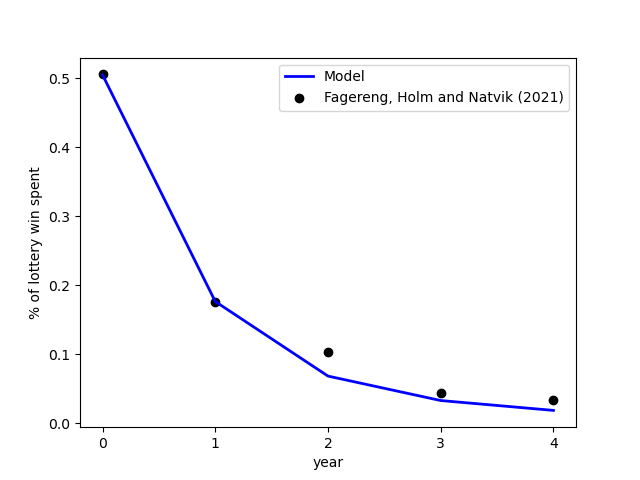
\includegraphics[width=\linewidth]{\econtexRoot/Code/HA-Models/Target_AggMPCX_LiquWealth/Figures/AggMPC_LotteryWin_comparison}
    \caption{Share of lottery win spent}
    \notinsubfile{\label{fig:aggmpclotterywin}}
  \end{subfigure}
  \begin{subfigure}[b]{.48\linewidth}
    \centering
    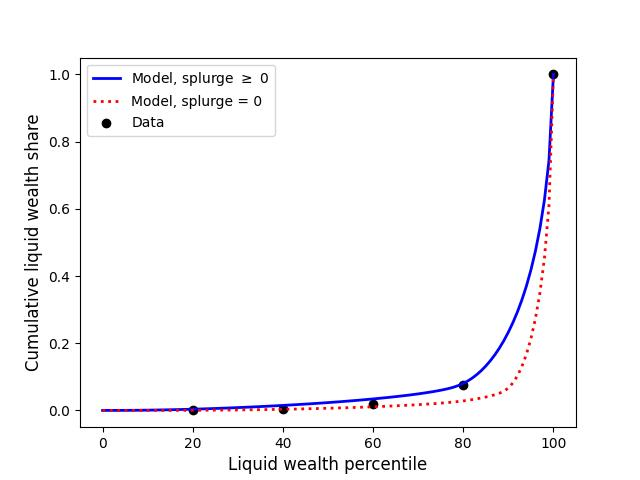
\includegraphics[width=\linewidth]{\econtexRoot/Code/HA-Models/Target_AggMPCX_LiquWealth/Figures/LiquWealth_Distribution_comparison}
    \caption{Distribution of liquid wealth}
    \notinsubfile{\label{fig:liquwealthdistribution}}
  \end{subfigure}%
  \caption{Marginal propensity to consume over time and the liquid wealth distribution in the model and the data}
  \notinsubfile{\label{fig:splurge_estimation}}
  \parbox{16cm}{\small \vspace{.15cm} \textbf{Note}: Panel (a) shows the fit of the model to the dynamic consumption response estimated in \citet{fagereng_mpc_2021}; see their figure~A5.
Panel (b) shows the fit of the model to the distribution of liquid wealth (see Section~\ref{sec:SCFdata} for the definition) from the 2004 SCF.\normalsize}
\end{figure}


% \newcommand{\iMPC}{\econtexRoot/Code/HA-Models/Target_AggMPCX_LiquWealth/Figures/AggMPC_LotteryWin_comparison}
% \newcommand{\LiqDist}{\econtexRoot/Code/HA-Models/Target_AggMPCX_LiquWealth/Figures/LiquWealth_Distribution_comparison}
% \begin{figure}[htb]
%   \ifdefined\HCode
%     \HCode{<div style="text-align: center;">}
%   \fi
%   \centering
%   \begin{tabular*}{\textwidth}{@{\extracolsep{\fill}}cc@{}}
%     \ifdefined\HCode
%       \HCode{<div style="display: flex; flex-direction: column; align-items: center; width: 48\%;">}
%     \fi
%     \subfloat[Share of lottery win spent\label{fig:aggmpclotterywin}]{%
%       \ifdefined\HCode
%         \includegraphics[width=\linewidth]{\iMPC}
%       \else
%         \includegraphics[width=0.48\textwidth]{\iMPC}
%       \fi
%     }
%     \ifdefined\HCode
%       \HCode{</div>}
%     \fi
%     &
%     \ifdefined\HCode
%       \HCode{<div style="display: flex; flex-direction: column; align-items: center; width: 48\%;">}
%     \fi
%     \subfloat[Distribution of liquid wealth\label{fig:liquwealthdistribution}]{%
%       \ifdefined\HCode
%         \includegraphics[width=\linewidth]{\LiqDist}
%       \else
%         \includegraphics[width=0.48\textwidth]{\LiqDist}
%       \fi
%     }
%     \ifdefined\HCode
%       \HCode{</div>}
%     \fi
%   \end{tabular*}
%   \ifdefined\HCode
%     \HCode{<figcaption style="text-align: center; width: auto; max-width: 800px;">}
%   \fi
%   \caption{Targets and model moments from the estimation}
%   \notinsubfile{\label{fig:splurge_estimation}}
%   \ifdefined\HCode
%     \HCode{<div style="text-align: justify; width: 16cm;  margin: 1em auto 0 auto;">}
%   \fi

% \parbox{14cm}{
%   \footnotesize \vspace{.15cm} Panel (a) shows the fit of the model to the dynamic consumption response estimated in \citet{fagereng_mpc_2021}; see their figure~A5. Panel (b) shows the fit of the model to the distribution of liquid wealth (see Section~\ref{sec:SCFdata} for the definition) from the 2004 SCF.\normalsize}
% \end{figure}

\begin{table}[t]
  \center
  \begin{tabular}{@{}lcccccc@{}} 
\toprule 
                  & \multicolumn{5}{c}{MPC} &   \\   
                  &  1st WQ  & 2nd WQ  & 3rd WQ & 4th WQ  & Agg  &  K/Y  \\  \midrule 
Model &0.27 & 0.49 & 0.60 & 0.66 & 0.50 & 6.59 \\ 
Data &0.39 & 0.39 & 0.55 & 0.66 & 0.51 & 6.60 \\ 
\end{tabular}  

  \caption{Marginal propensities to consume across wealth quartiles and the total population as well as the wealth to income ratio, in the model and according to the data}
  \notinsubfile{\label{tab:MPC_WQ}}
\end{table}


For this estimation exercise, the remaining model parameters are calibrated to reflect the Norwegian economy.
Specifically, we set the real interest rate to $2$ percent annually and the unemployment rate to $4.4$ percent, in line with \citet{aursland_state-dependent_2020}.
The quarterly probability to survive is calibrated to $1-1/160$, reflecting an expected working life of 40 years.
Aggregate productivity growth is set to $1$ percent annually, following \citet{kravik_navigating_2019}.
The unemployment net replacement rate is calibrated to $60$ percent, following \citet{oecd_net_2020}.
Finally, we set the real interest rate on liquid debt to $13.6$ percent, following data from the Norwegian debt registry \citet{gjeldsregistret_nokkeltall_2022}.\footnote{Specifically, we determine the average volume-weighted interest rate on liquid debt, which consists of consumer loans, credit and payment card debt and all other unsecured debt.
We use data from December 2019.
Note that although these data let us pin down aggregate quantities, they do not solve the issue referred to in footnote~\ref{foot:liqwealth}, since we cannot link them to the tax registry at the individual level.
We set the borrowing limit on liquid debt to zero.}

Estimates of the standard deviations of the permanent and transitory shocks are taken from \citet{crawleyParsimonious}, who estimate an income process on administrative data for Norwegian males from 1971 to 2014.
The estimated annual variances for the permanent and transitory shocks are 0.004 and 0.033, respectively.\footnote{As shown in \citet{crawleyParsimonious}, an income process of the form that we use here is more accurately estimated using moments in levels not differences.
Hence, we take the numbers from column 3 of Panel C in their table 4.} As in \citet{carroll2020sticky}, these are converted to quarterly values by multiplying the permanent and transitory shock variances by $1/4$ and $4$, respectively.
Thus, we obtain quarterly standard deviations of $\sigma_\psi=0.0316$ and $\sigma_\xi=0.363$.

Using the calibrated model, we simulated unexpected lottery winnings and calculate the share of the lottery spent in each year.
Specifically, each simulated agent receives a lottery win in a random quarter of the first year of the simulation.
The size of the lottery win is itself random and spans the range of lottery sizes found in \citet{fagereng_mpc_2021}.
The estimation procedure minimizes the distance between the target and model moments by selecting the splurge factor and the distribution of discount factors in the population, where the latter are assumed to be uniformly distributed in the range $[\beta-\nabla, \beta+\nabla]$.
We approximate the uniform distribution of discount factors with a discrete approximation and let the population consist of eight different types.

The estimation yields a splurge factor of $0.249$ and a distribution of discount factors described by $\beta = 0.968$ and $\nabla=0.0578$.
Given these estimated parameters and the remaining calibrated ones, the model is able to replicate the time path of consumption in response to a lottery win from \citet{fagereng_mpc_2021} and the targeted distribution of liquid wealth very well, see Figure \ref{fig:splurge_estimation}.
Also, the targeted moments discussed in Table \ref{tab:MPC_WQ} are captured relatively well.
In particular, the model is able to account for the empirical fact that MPC consume for high-wealth agents is substantially larger than zero, see the first column.




 

\hypertarget{data-on-permanent-income-liquid-wealth-and-education}{}\par\subsection{Data on permanent income, liquid wealth, and education}
\notinsubfile{\label{sec:SCFdata}}

Before we move on to the parameterization of the full model, we describe in detail the data that we use to get measures of permanent income, liquid wealth, and the division of households into educational groups in the United States.
We use data on the distribution of liquid wealth from the 2004 wave of the SCF.
We restrict our attention to households where the head is of working age, which we define to be in the range from 25 to 62.
The SCF-variable ``normal annual income'' is our measure of the household's permanent income, and, to exclude outliers, we drop the observations that make up the bottom 5 percent of the distribution of this variable.
The smallest value of permanent income for households in our sample is thus \$16,708.


Liquid wealth is defined as in \cite{kaplan2014model} and consists of cash, money market, checking, savings, and call accounts; directly held mutual funds; and stocks and bonds.
We subtract off liquid debt, which is the revolving debt on credit card balances.
Note that the SCF does not contain information on cash holdings, so these are imputed with the procedure described in Appendix B.1 of \cite{kaplan2014model}, which also describes the credit card balances that are considered part of liquid debt.
We drop any households that have negative liquid wealth.


Households are classified into three educational groups.
The first group, ``Dropout,'' applies to households where the head of household has not obtained a high school diploma; the second group, ``Highschool,'' includes heads of households who have a high school diploma and those who, in addition, have some years of college education without obtaining a bachelor's degree; and the third group, ``College,'' consists of heads of households who have obtained a bachelor's degree or higher.
With this classification of the education groups, the Dropout group makes up $9.3$ percent of the population, the Highschool group $52.7$ percent, and the College group $38.0$ percent.


With our sample selection criteria, we are left with a sample representing about 61.3 million U.S.
households.

\subsection{Parameters in the full model}
\notinsubfile{\label{sec:paramsFull}}

With households classified into the three education groups using the SCF data, we proceed to set the parameters of the model as follows.
First, we calibrate a set of parameters that apply to all types of houesholds in the model.
Second, we calibrate another set of parameters that are specific to each education group to capture broad differences across these groups.
Finally, given the calibrated parameters we estimate discount factor distributions for each education group that allow us to match the distribution of liquid wealth in each group.


The model is a simplified model for households in that we do not take into account heterogeneity across household size or composition.
The households are ex-ante heterogeneous in their subjective discount factors as well as their level of education.
We classify the education level of the household based on the education of the head of the household, and we typically think of individual characteristics as applying to that person.


A period in the model is one quarter.
This choice makes it realistic to consider stimulus policies that are implemented in the same period as a recession starts.


\subsubsection{Calibrated parameters --- Normal times} 
\notinsubfile{\label{sec:calib}}

Table~\ref{tab:calibration} presents our calibration of the model parameters in normal times. Panel~A lists parameters that are calibrated equally across all types in the model, and Panel~B lists parameters in the model that are education specific. In the next subsection we present how certain model parameters are changes when the economy enters a recession. 

\textbf{Preferences, survival and interest rates.} All households are assumed to have a coefficient of relative risk aversion equal to $\gamma=2$.
We also assume that all households have the same propensity to splurge out of transitory income gains and set $\varsigma=0.249$, the value estimated in section~\ref{sec:splurge}.
However, each education group is divided into types that differ in their subjective discount factors.
The distributions of discount factors for each education group are estimated to fit the distribution of liquid wealth within that group, and this estimation is described in detail in section~\ref{sec:estimBetas}.
Regardless of type, households face a constant survival probability each quarter.
This probability is set to $1-1/160$, reflecting an expected working life of 40 years.
The real interest rate on households' savings is set to $1$ percent per quarter.



\afterpage{
  \thispagestyle{empty}
  \begin{table}[p]
    \caption{Calibrated Model Parameters --- Normal times}
    \center
%    \begin{center}
      \begin{tabular}{c}
        \begin{tabular}{lcd{3}} 
          \toprule
          \multicolumn{3}{l}{Panel (A) Parameters that apply to all types} \\ \midrule
          Parameter & Notation & \text{Value} \\ \midrule 
          Risk aversion & $\gamma$ & 2.0 \\ 
          Splurge & $\varsigma$ & 0.249 \\ 
          Survival probability, quarterly & $1-D$ & 0.994 \\
          Risk free interest rate, quarterly (gross) & $R$ & 1.01 \\ 
          Standard deviation of transitory shock & $\sigma_\xi$ & 0.346 \\
          Standard deviation of permanent shock & $\sigma_\psi$ & 0.0548 \\ 
          Unemployment benefits replacement rate (share of PI) & $\rho_b$ & 0.7 \\ 
          Unemployment income w/o benefits (share of PI) & $\rho_{nb}$ & 0.5 \\ 
          Avg. duration of unemp. benefits in normal times (quarters) & & 2 \\
          Avg. duration of unemp. spell in normal times (quarters) & & 1.5 \\
          Probability of leaving unemployment & $\pi_{ue}$ & 0.667 \\ 
          Consumption elasticity of aggregate demand effect & $\kappa$ & 0.3 
          \\ \bottomrule 
        \end{tabular} \\ \\

        \begin{tabular}{lccc}
          \toprule 
          \multicolumn{4}{l}{Panel (B) Parameters calibrated for each education group} \\ \midrule
          & Dropout & Highschool & College \\ \midrule
          Percent of population & \phantom{0}9.3 & 52.7 & 38.0 \\ 
          Avg. quarterly PI of ``newborn'' agent (\$1000) & \phantom{0}6.2 & 11.1 & 14.5 \\
          Std. dev. of $\log($PI$)$ of ``newborn'' agent & 0.32 & 0.42 & 0.53 \\
          Avg. quarterly gross growth rate of PI ($\Gamma_e$) & 1.0036 & 1.0045 & 1.0049 \\
          Unemployment rate in normal times (percent) & \phantom{0}8.5 & \phantom{0}4.4 & \phantom{0}2.7 \\ 
          Probability of entering unemployment ($\pi_{eu}^{e}$, percent) & \phantom{0}6.2 & \phantom{0}3.1 & \phantom{0}1.8 
          \\ \bottomrule 
        \end{tabular} \\
        \ifdefined\HCode
        \HCode{<div style="text-align: justify; width: 16cm;  margin: 1em auto 0 auto;">}
        \fi
        \parbox{16cm}{\footnotesize \vspace{.25cm} \textbf{Note}: The first three rows show numbers from the 2004 SCF.
The fourth row are averages of growth rates from \cite{carroll2020modeling}.
The fifth row are numbers for 2004 from the Bureau of Labor Statistics, and the sixth row are calculated from these unemployment rates.\normalsize}
%        \\ \\
%
%        \begin{tabular}{lc}
%          \toprule 
%          \multicolumn{2}{l}{Panel (C) Parameters describing policy experiments} \\ \midrule 
%          Parameter & Value \\ \midrule 
%          Change in unemployment rates in a recession & $\times 2$ \\ 
%          Expected unemployment spell in a recession & 4 quarters \\ 
%          Average length of recession & 6 quarters \\ 
%          Size of stimulus check & \$1,200 \\ 
%          PI threshold for reducing check size & \$100,000 \\ 
%          PI threshold for not receiving check & \$150,000 \\ 
%          Extended unemployment benefits & 4 quarters \\
%          Length of payroll tax cut & 8 quarters \\ 
%          Income increase from payroll tax cut & 2 percent \\ 
%          Belief (probability) that tax cut is extended & 50 percent 		
%          \\ \bottomrule
%        \end{tabular} 

      \end{tabular}
%    \end{center}
    \begin{tabular}{p{16cm}}
%      \parbox{16cm}{
      \medskip
      \small Panel (A) shows parameters calibrated the same for all types. Panel (B) shows parameters calibrated for each education group. ``PI'' refers to permanent income.
      % Panel (C) shows the numbers describing how we model a recession and the three policies we consider.}
      \end{tabular}
    \notinsubfile{\label{tab:calibration}}
  \end{table}
  \clearpage
}

\textbf{Labor market risk while employed.} When consumers are born, they receive an initial level of permanent income.
This initial value is drawn from a log-normal distribution that depends on the education level the household is born with.
For each education group, the parameters of the distribution are determined by the mean and standard deviation of log-permanent income for households in that group where the head of the household is of age 25 in the SCF 2004.
For the Dropout group, the mean initial value of quarterly permanent income is \$6,200; for the Highschool group, it is \$11,100; and for the College group, it is \$14,500.
The standard deviations of the log-normal distributions for each group are, respectively, $0.32$, $0.42$, and $0.53$.


While households remain employed, their income is subject to both permanent and transitory idiosyncratic shocks.
These shocks are distributed equally for the three education groups.
The standard deviations of these shocks are taken from \cite{carroll2020sticky}, who set the standard deviations of the transitory and permanent shocks to $\sigma_\xi=0.346$ and $\sigma_\psi=0.0548$, respectively.


Permanent income also grows, on average, with a growth rate $\Gamma_{e(i)}$ that depends on the level of education.
These average growth rates are based on numbers from \cite{carroll2020modeling}, who construct age-dependent expected permanent income growth factors using numbers from \cite{cagetti2003wealth} and fit the age-dependent numbers to their life-cycle model.
We construct the quarterly growth rates of permanent income in our perpetual-youth model by taking the average of the age-dependent growth rates during a household's working life.
The average gross quarterly growth rates that we obtain for the three education groups are then $\Gamma_d=1.0036$, $\Gamma_h=1.0045$, and $\Gamma_c=1.0049$.

\textbf{Unemployment.} Consumers also face the risk of becoming unemployed and will then have access to unemployment benefits for a certain period.
The parameters describing the unemployment benefits in normal times are based on the work of \cite{rothstein2017scraping}, who study the effects on household income of unemployment and of running out of eligibility for benefits.
The unemployment benefits replacement rate is thus set to $\rho_b=0.7$ for all households, and when benefits run out, the unemployment replacement rate without any benefits is set to $\rho_{nb}=0.5$.
These replacement rates are set as a share of the households' permanent income and are based on the initial drop in income upon entering an unemployment spell, presented in figure~3 in \cite{rothstein2017scraping}.\footnote{See the lines for their UI exhaustee sample including and excluding UI income.
\cite{rothstein2017scraping} also point out that ``UI benefits replace about 40 percent of the lost earnings on average'' (page 894).
For a household with two income earners with equal income, these findings would mean that income drops to 70 percent when one earner becomes unemployed and to 50 percent when benefits run out.
In this paper we ignore several of the channels studied by \cite{rothstein2017scraping} such as within household insurance and other social programs that can provide income even after UI benefits have run out.} 

The duration of unemployment benefits in normal times is set to two quarters, so that our Markov transition matrix $\Pi$ has four states.
This length of time corresponds to the mean duration of unemployment benefits across U.S.
states from 2004 to mid-2008 of 26 weeks, reported by \cite{rothstein2017scraping}.


The probability of transitioning out of unemployment is set to match the average duration of an unemployment spell in normal times.
In data from the Bureau of Labor Statistics, this average duration was 19.6 weeks or 1.5 quarters in 2004. We do not have data on  education-specific duration rates, however, so we set the average duration of unemployment to 1.5 quarters for all households. This implies that the transition probability from unemployment to employment is set to $\pi_{ue}=2/3$.


The Bureau of Labor Statistics provide data on unemployment rates for different education groups, and we match the average rate in each group in 2004 by setting an education-specific probability of transitioning from employment into unemployment.
Note that this calibration strategy is consistent with the results in \citet{mincer1991education} who finds that the main difference between education groups is in the incidence of unemployment, and not its duration.\footnote{\citet{mincer1991education} states that ``the reduction of the incidence of unemployment [at higher education levels] is found to be far more important than the reduced duration of unemployment in creating the educational differentials in unemployment rates'' (page 1).} More recent work by \citet{elsby2010labor} includes data upto 2009 and echoes \citeauthor{mincer1991education}'s results.


The average unemployment rate in 2004 was 8.5 percent for the Dropout group, 4.4 percent for the Highschool group, and 2.7 percent for the College group.
These values imply that the probabilities of transitioning into unemployment in normal times are $\pi_{eu}^d=6.2$ percent, $\pi_{eu}^h=3.1$ percent, and $\pi_{eu}^c=1.8$ percent, respectively.\footnote{Also note that the probability of transitioning from employment to unemployment is the probability of a job separation times the conditional probability of unemployment given a job separation.
\citet{mincer1991education} reports that both of these are lower for higher education levels.
For our calibration, this means that a higher job finding rate \textit{within} the quarter of the job separation for more educated workers translates	into a lower probability of transitioning from employment to unemployment during a quarter.
In that sense, our calibration is consistent with short-term job-finding rates being higher for more educated workers.}

Finally, the strength of the aggregate demand effect in recessions is determined by the consumption elasticity of productivity.
We follow \cite{kmpHandbook2016} and set this to $\kappa=0.3$.


\subsubsection{Calibrated parameters --- Recession} 
\notinsubfile{\label{sec:calibRecession}}

Table~\ref{tab:calibrationRecession} shows the model parameters that change when a recession hits. Panel~A shows the change in two parameters that apply to all types, and Panel~B shows changes in some parameters that differ across education groups. For completeness, panel~C summarizes the remaining parameters describing how we model a recession and the three policies we consider as potential responses to a recession.

The two immediate changes that occur at the outset of a recession is that the unemployment rate doubles for all education groups, and the expected duration of an unemployment spell increases from $1.5$ to $4$ quarters. The duration of unemployment is the same across the three education groups, and this implies that the probability of leaving unemployment is set to $\pi_{ue} = 0.25$ in a recession. 

The increase in the expected duration of unemployment combined with the doubling of the education-specific unemployment rates pin down new values for the probabilities of transitioning from employment to unemployment during the recession. Due to the large increase in the unemployment duration, the values that we obtain end up being slightly smaller than those transition probabilities in normal times. The probability $\pi_{eu}$ in a recession is set to $5.1$ percent for the Dropout group, $2.4$ percent for the Highschool group, and $1.4$ for the College group. 

Our calibration of the transition probabilities between employment and unemployment during a recession are thus broadly in line with the results of \citet{elsby2010labor}. They find that unemployment duration does not vary much between education groups and that the flow from unemployment to employment drops sharply for all groups in a recession. The flow into unemployment is more stable, but they find that it tends to increase a little bit in recessions.\footnote{See the bottom row of Figure~8 in \citet{elsby2010labor} for these results.} This differs from the small decrease in the transition probabilities from employment into unemployment that our calibration strategy implies, which follows from our choice of targeting a doubling of the unemployment rate for each group rather than an even larger increase. 

  \begin{table}[p]
	\caption{Calibrated Model Parameters --- Recession}
	\center
	%    \begin{center}
		\begin{tabular}{c}
			\begin{tabular}{lcd{3}} 
				\toprule
				\multicolumn{3}{l}{Panel (A) Parameters that apply to all types} \\ \midrule
				Parameter & Notation & \text{Value} \\ \midrule 
				Avg. duration of unemp. spell in a recession (quarters) & & 4 \\
				Probability of leaving unemployment in a recession & $\pi_{ue}$ & 0.25 
				\\ \bottomrule 
			\end{tabular} \\ \\
			
			\begin{tabular}{lccc}
				\toprule 
				\multicolumn{4}{l}{Panel (B) Parameters calibrated for each education group} \\ \midrule
				& Dropout & Highschool & College \\ \midrule
				Unemployment rate at the start of a recession (percent) & \phantom{0}17.0 & \phantom{0}8.8 & \phantom{0}5.4 \\ 
				Probability of entering unemployment ($\pi_{eu}^{e}$, percent) & \phantom{0}5.1 & \phantom{0}2.4 & \phantom{0}1.4 
				\\ \bottomrule 
			\end{tabular} \\ \\
%			\ifdefined\HCode
%			\HCode{<div style="text-align: justify; width: 16cm;  margin: 1em auto 0 auto;">}
%			\fi
%			\parbox{16cm}{\footnotesize \vspace{.25cm} \textbf{Note}: Education-specific model parameters that change in a recession.\normalsize}
%			\\ \\
			
			\begin{tabular}{lc}
				\toprule 
				\multicolumn{2}{l}{Panel (C) Parameters describing policy experiments} \\ \midrule 
				Parameter & Value \\ \midrule 
				%Change in unemployment rates in a recession & $\times 2$ \\ 
				%Expected unemployment spell in a recession & 4 quarters \\ 
				Average length of recession & 6 quarters \\ 
				Size of stimulus check & \$1,200 \\ 
				PI threshold for reducing check size & \$100,000 \\ 
				PI threshold for not receiving check & \$150,000 \\ 
				Extended unemployment benefits & 4 quarters \\
				Length of payroll tax cut & 8 quarters \\ 
				Income increase from payroll tax cut & 2 percent \\ 
				Belief (probability) that tax cut is extended & 50 percent 		
				\\ \bottomrule
			\end{tabular} 
			
		\end{tabular}
		%    \end{center}
	\begin{tabular}{p{16cm}}
		%      \parbox{16cm}{
			\medskip
			\small Panel (A) shows the parameters that apply to all types that change in a recession. Panel (B) shows the education-specific model parameters that change in a recession. Panel (C) shows numbers further describing how we model a recession and the three policies we consider. ``PI'' refers to permanent income.
			% }
	\end{tabular}
	\notinsubfile{\label{tab:calibrationRecession}}
\end{table}




\hypertarget{estimating-the-discount-factor-distributions}{}\par\subsubsection{Estimating the discount factor distributions} 
\notinsubfile{\label{sec:estimBetas}}

Discount factor distributions are estimated separately for each education group to match the distribution of liquid wealth for households in that group.
To do so, we let each education group consist of types that differ in their subjective discount factor,~$\beta$.
The discount factors within each group $e\in \{d, h, c\}$ are assumed to be uniformly distributed in the range $[\beta_e-\nabla_e, \beta_e+\nabla_e]$.
The parameters $\beta_e$ and $\nabla_e$ are chosen for each group separately to match the median liquid-wealth-to-permanent-income ratio and the $\nth{20}$, $\nth{40}$, $\nth{60}$, and $\nth{80}$ percentile points of the Lorenz curve for liquid wealth for that group.
We approximate the uniform distribution of discount factors with a discrete approximation and let each education group consist of seven different types.

Panel~A of table~\ref{tab:estimBetas} shows the estimated values of $(\beta_e, \nabla_e)$ for each education group.
The panel also shows the minimum and maximum values of the discount factors we actually use in the model when we use a discrete approximation with seven values to approximate the uniform distribution of discount factors.
Panel~B of table~\ref{tab:estimBetas} shows that with these estimated distributions, we can exactly match the median liquid-wealth-to-permanent-income ratios for each education group.
Figure~\ref{fig:LorenzPts} shows that with the estimated distributions, the model quite closely matches the distribution of liquid wealth within each education group as well as for the population as a whole.
Thus, our model does not suffer from the ``missing middle'' problem, identified in \cite{kaplanMPC2022}, in which the middle of the wealth distribution has too little wealth.

%Our model avoids this problem for two reasons: (1) The splurge pushes up MPCs relative to wealth, and (2) we calibrate to liquid wealth rather than total wealth.

\begin{table}[th]
  \begin{center}
    \begin{tabular}{l}
      \begin{tabular}{lccc}
        \multicolumn{4}{l}{Panel (A) Estimated discount factor distributions} \\ \midrule
        & Dropout & Highschool & College \\ \midrule
        $(\beta_e, \nabla_e)$ & (0.719, 0.318) & (0.911, 0.137) & (0.983, 0.014) \\
        (Min, max) in approximation & (0.447, 0.991) & (0.793, $0.990^*$) & (0.971, 0.995) \\
        \midrule 
      \end{tabular} \\ \\ 
      
      \begin{tabular}{lccc}
        \multicolumn{4}{l}{Panel (B) Estimation targets} \\ \midrule
        & Dropout & Highschool & College \\ \midrule
        Median LW/ quarterly PI (data, percent) & 4.64 & 30.2 & 112.8 \\ 
        Median LW/ quarterly PI (model, percent) & 4.64 & 30.2 & 112.8 %\\
        %         $[20,40,60,80]$ pctiles of Lorenz curve (data) & $[0, 0.01, 0.6, 3.6]$ & $[0.06, 0.6, 3.0, 11.6]$ & $[0.2, 0.9, 3.3, 10.3]$ \\
        %         $[20,40,60,80]$ pctiles of Lorenz curve (model) & $[0.0, 0.0, 0.6, 3.6]$ & $[0.05, 0.8, 3.1, 11.5]$ & $[0.3, 1.3, 3.6, 10.1]$
        \\ \midrule 
      \end{tabular} \\ \\ 
    \end{tabular}
    \caption{Estimated discount factor distributions and estimation targets}
    \notinsubfile{\label{tab:estimBetas}}
    \parbox{16cm}{\small \vspace{.15cm} \textbf{Note}: Panel (A) shows the estimated parameters of the discount distributions for each education group.
It also shows the minimum and maximum values we use in our discrete approximation to the uniform distribution of discount factors for each group.
The $*$ indicates that the highest value in the uniform distribution of discount factor values violates the growth impatience condition (GIC) and has been replaced.
Panel (B) shows the weighted median ratio of liquid wealth to permanent income from the 2004 SCF and in the model.
In the annual data from the SCF, the annual PI is divided by 4 to obtain a quarterly number.\normalsize}
  \end{center}
\end{table}

One point we should note concerns the estimated discount factor distribution for the Highschool group.
Panel~A of table~\ref{tab:estimBetas} reports values of $\beta_h=0.911$ and $\nabla_h=0.137$.
With these values, the largest discount factors in our discrete approximation of the uniform distribution in the range $[\beta_h-\nabla_h, \beta_h+\nabla_h]$ would be greater than $1$.
More importantly, the value would violate the Growth Impatience Condition (GIC), discussed in \cite{carroll2022theoretical}.
(The GIC is required to prevent the ratio of total wealth to total income of any group from approaching infinity.
It does this by making sure that the growth of wealth of the group is less than or equal to the growth of income.)
We replace values violating the GIC with values close to the upper bound on $\beta$ imposed by the GIC.
In panel~A of table~\ref{tab:estimBetas} the largest value is marked by a $*$ to indicate that it has been replaced to avoid violating the GIC.
We always impose that the GIC is satisfied in the estimation of the discount factor distributions, but for the baseline parameter values it is only binding for the Highschool group.
Thus, the estimation can select a large value of $\nabla_h$ without violating the constraint.\footnote{The constraint is imposed by calculating a discount factor $\beta^{\text{GIC}}$ where the GIC holds with equality.
Then the estimation can pick how close to this value the largest discount factor is by estimating $x$ and setting the largest discount factor to $\exp(x)/(1+\exp(x)) \beta^{\text{GIC}}$.} 

\begin{figure}[th]
  \begin{center}
    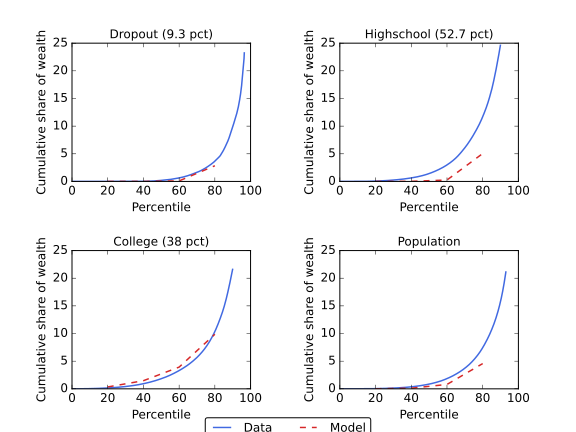
\includegraphics[width=.9\textwidth]{\econtexRoot/Figures/LorenzPoints_CRRA_2.0_R_1.01}
    \caption{Distributions of liquid wealth within each education group and for the whole population from the 2004 Survey of Consumer Finances and from the model with estimated discount factor distributions}
    \notinsubfile{\label{fig:LorenzPts}}
    \parbox{16cm}{\small \vspace{.15cm} \textbf{Note}: The discount factor distributions are estimated separately for each education group to fit the median liquid-wealth-to-permanent-income ratio and the $\nth{20}$, $\nth{40}$, $\nth{60}$, and $\nth{80}$ percentile points of the Lorenz curve for liquid wealth for that group. The ``Population'' panel compares the wealth distribution that results from pooling the three groups in the model to the overall wealth distribution in the data.\normalsize}
  \end{center}
\end{figure}

Also, note that several of the types in the Dropout group have very low discount factors and are very impatient.
In this way, the model fits the feature of the data for the Dropout group that the bottom quintiles do not save at all and do not accumulate any liquid wealth.
Very low estimates for discount factors are in line with those obtained in the literature on payday lending.\footnote{See, for example, \cite{skiba2008payday}, who estimate two-week discount rates of $21$ percent, and \cite{allcott2021high}, who estimate an initial period discount factor between $0.74$ and $0.83$ in a model where a period is eight weeks long.
Both of these papers use quasi-hyperbolic preferences, so the estimates are not directly comparable with parameters in our model.
Nevertheless, they support the point that very high discount rates are necessary to model the part of the population that takes out payday loans at very high interest rates.} 

\hypertarget{non-targeted-moments}{}\par\subsubsection{Implications for non-targeted moments} 
\notinsubfile{\label{sec:nonTargetedMoments}}

Before we move on to compare different consumption stimulus policies in the calibrated model, we also report implications of the model for some non-targeted moments.
Panel~A of table~\ref{tab:nonTargetedMoments} shows the wealth distribution across the three education groups in the data and in the model.
The model matches these shares quite closely, which may not be surprising given that we calibrate the size of each group and we manage to fit the wealth distribution within each group separately.
The panel also reports the average marginal propensity to consume for the different groups.
To be comparable to numbers reported in \citet{fagereng_mpc_2021}, these are calculated as the average MPC in the year of a lottery win.
Lottery wins occur in a random quarter of the year that differs across individuals.
The MPC for an individual depends on the spending pattern after the win, and these are averaged across individuals within each education group.


Panel~B of table~\ref{tab:nonTargetedMoments} shows similar numbers to Panel~A, sorted by quartiles of the liquid wealth distribution instead of education groups.
Our model yields a slightly more concentrated liquid wealth distribution than in the data.
However, it does produce a fairly high MPC even for households in the highest quartile of the liquid wealth distribution.
This is consistent with the results found in the Norwegian data by \citet{fagereng_mpc_2021}, but also with recent results in \citet{graham2024mental}.
In an administrative dataset from a large US financial institution, they find that the spending response to an income receipt is large across the distribution of liquid asset holdings.
In our model, we obtain this result due to the inclusion of the splurge factor.
As shown in Appendix~\ref{app:Model_without_splurge}, the model is not able to generate a high MPC for the highest wealth quartile without splurge consumption.


\begin{table}[th]
    \centering
    \begin{tabular*}{\textwidth}{@{\extracolsep{\fill}}c@{}}
        \begin{tabular}{lcccc}
            \multicolumn{5}{c}{Panel (A) Non-targeted moments by education group} \\ \midrule
            & Dropout & Highschool & College & Population \\ \midrule
            Percent of liquid wealth (data) & 0.8 & 17.9 & 81.2 & 100 \\
            Percent of liquid wealth (model) & 1.1 & 21.9 & 77.0 & 100 \\
            \makecell[l]{Avg. lottery-win-year MPC \\ (model, incl. splurge)} & 0.78 & 0.61 & 0.38 & 0.54
            \\ \bottomrule 
        \end{tabular} \\ \\

      \vspace{2em}
      
        \begin{tabular}{lcccc}
            \multicolumn{5}{c}{Panel (B) Non-targeted moments by wealth quartile} \\ \midrule
             & WQ 4 & WQ 3 & WQ 2 & WQ 1 \\ \midrule
            Percent of liquid wealth (data) & 0.14 & 1.60 & 8.51 & 89.76 \\
            Percent of liquid wealth (model) & 0.09 & 0.96 & 4.55 & 94.40 \\
            \makecell[l]{Avg. lottery-win-year MPC \\ (model, incl. splurge)} & 0.78 & 0.63 & 0.44 & 0.31
            \\ \bottomrule 
        \end{tabular}
    \end{tabular*}
    \caption{Model fit with respect to non-targeted moments}
    \notinsubfile{\label{tab:nonTargetedMoments}}
    \parbox{16cm}{\small \vspace{.15cm} \textbf{Note}: Panel (A) shows percent of liquid wealth held by each education group in the 2004 SCF and in the model.
It also shows the average MPCs after a lottery win for each education group.
The MPCs are calculated for each individual for the year of a lottery win, taking into account that the win takes place in a random quarter of the year that differs across individuals.
The MPCs are averaged across individuals within each education group.
Panel~(B) shows the same numbers for the population sorted into different quartiles of the liquid wealth distribution.\normalsize}
  \end{table}
  
% \begin{table}[th]
% 	\begin{center}
% 		\begin{tabular}{l}
% 			\begin{tabular}{lcccc}
% 				\multicolumn{5}{l}{Panel (A) Non-targeted moments by education group} \\ \midrule
% 				& Dropout & Highschool & College & Population \\ \midrule
% 				Percent of liquid wealth (data) & 0.8 & 17.9 & 81.2 & 100 \\
% 				Percent of liquid wealth (model) & 1.1 & 21.9 & 77.0 & 100 \\
% 				\makecell[l]{Avg. lottery-win-year MPC \\ (model, incl. splurge)} & 0.78 & 0.61 & 0.38 & 0.54
% 				\\ \bottomrule 
% 			\end{tabular} \\ \\ 
			
% 			\begin{tabular}{lcccc}
% 				\multicolumn{5}{l}{Panel (B) Non-targeted moments by wealth quartile} \\ \midrule
% 				 & WQ 4 & WQ 3 & WQ 2 & WQ 1 \\ \midrule
% 				Percent of liquid wealth (data) & 0.14 & 1.60 & 8.51 & 89.76 \\
% 				Percent of liquid wealth (model) & 0.09 & 0.96 & 4.55 & 94.40 \\
% 				\makecell[l]{Avg. lottery-win-year MPC \\ (model, incl. splurge)} & 0.78 & 0.63 & 0.44 & 0.31
% 				\\ \bottomrule 
% 			\end{tabular}
% 		\end{tabular}
% 		\caption{Implications for non-targeted moments}
% 		\notinsubfile{\label{tab:nonTargetedMoments}}
% 		\parbox{16cm}{\small \vspace{.15cm} \textbf{Note}: Panel (A) shows percent of liquid wealth held by each education group in the 2004 SCF and in the model. It also shows the average MPCs after a lottery win for each education group. The MPCs are calculated for each individual for the year of a lottery win, taking into account that the win takes place in a random quarter of the year that differs across individuals. The MPCs are averaged across individuals within each education group. Panel~(B) shows the same numbers for the population sorted into different quartiles of the liquid wealth distribution.\normalsize}
% 	\end{center}
% \end{table}

Finally, we consider the implications of our model for two different patterns of spending over time.
The first pattern is the dynamics of spending after a lottery win from \citeauthor{fagereng_mpc_2021}.
This pattern was used in the estimation of the splurge factor in section~\ref{sec:splurge}, but was not targeted when estimating the discount factor distributions for each education group in section~\ref{sec:estimBetas}.
Figure~\ref{fig:USaggmpclotterywin} shows that the model that is estimated taking the value of the splurge as given, results in a distribution of spending over time that is very similar to the one found in the Norwegian data.

\hypertarget{ganong-noel}{}

The second pattern concerns the dynamics of income and spending for households that become unemployed and remain unemployed long enough for unemployment benefits to expire.
Figure~\ref{fig:expiryUI} shows the pattern of income and spending for such households.
\citet{ganongConsumer2019} report the empirical result that nondurable spending drops by 12 percent the month when benefits expire.
Our quarterly model is broadly consistent with this, and the drop in spending the quarter after the expiry of UI benefits is 18 percent.


% \begin{figure}[htb]
%     \centering
%     \begin{minipage}[b]{.48\linewidth}
%         \centering
%         \includegraphics[width=\linewidth]{\econtexRoot/Figures/iMPCs_wSplEstimated}
%         \caption{Share of lottery win spent}
%         \notinsubfile{\label{fig:USaggmpclotterywin}}
%     \end{minipage}%
%     \hfill
%     \begin{minipage}[b]{.48\linewidth}
%         \centering
%         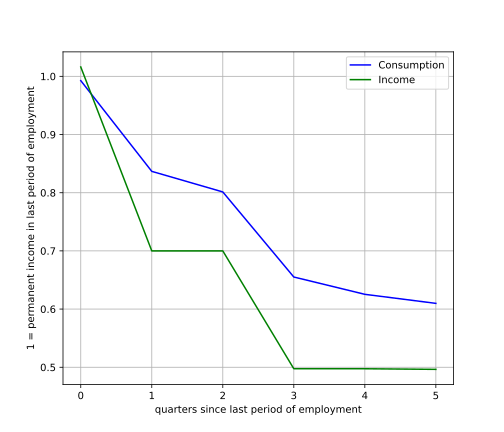
\includegraphics[width=\linewidth]{\econtexRoot/Code/HA-Models/FromPandemicCode/Figures/UnempSpell_Dynamics}
%         \caption{Spending upon expiry of UI benefits}
%         \notinsubfile{\label{fig:expiryUI}}
%     \end{minipage}
%     \caption{Untargeted moments}
%     \notinsubfile{\label{fig:untargetedMoments}}
%     \parbox{16cm}{\small \vspace{.15cm} \textbf{Note}: Panel (a) compares the dynamic consumption response in the model to the estimates in \citet{fagereng_mpc_2021}; see their Figure~A5. Panel (b) shows the evolution of income and spending for households who remain unemployed long enough for UI benefits to expire; see Figure~2 in \citet{ganongConsumer2019}.\normalsize}
% \end{figure}

\begin{figure}[htb]
    \centering
    \begin{subfigure}[b]{.48\linewidth}
        \centering
        \includegraphics[width=\linewidth]{\econtexRoot/Figures/iMPCs_wSplEstimated}
        \caption{Share of lottery win spent}
        \notinsubfile{\label{fig:USaggmpclotterywin}}
    \end{subfigure}%
    \begin{subfigure}[b]{.48\linewidth}
        \centering
        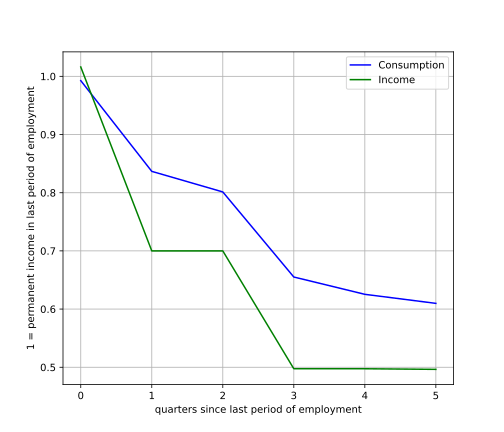
\includegraphics[width=\linewidth]{\econtexRoot/Code/HA-Models/FromPandemicCode/Figures/UnempSpell_Dynamics}
        \caption{Spending upon expiry of UI benefits}
        \notinsubfile{\label{fig:expiryUI}}
    \end{subfigure}
    \caption{Marginal propensity to consume over time and the spending upon expiry of UI benefits in the model}
    \notinsubfile{\label{fig:untargetedMoments}}
    \parbox{16cm}{\small \vspace{.15cm} \textbf{Note}: Panel (a) compares the dynamic consumption response in the model to the estimates in \citet{fagereng_mpc_2021}; see their Figure~A5.
Panel (b) shows the evolution of income and spending for households who remain unemployed long enough for UI benefits to expire; see Figure~2 in \citet{ganongConsumer2019}.\normalsize}
  \end{figure}
  
% \begin{figure}[htb]
%   \ifdefined\HCode
%     \HCode{<div style="text-align: center;">}
%   \fi
%   \centering
%   \begin{tabular*}{\textwidth}{@{\extracolsep{\fill}}cc@{}}
%     \ifdefined\HCode
%       \HCode{<div style="display: flex; flex-direction: column; align-items: center; width: 48\%;">}
%     \fi
%     \subfloat[Share of lottery win spent\label{fig:USaggmpclotterywin}]{%
%       \ifdefined\HCode
%         \includegraphics[width=\linewidth]{\econtexRoot/Figures/iMPCs_wSplEstimated}
%       \else
%         \includegraphics[width=0.48\textwidth]{\econtexRoot/Figures/iMPCs_wSplEstimated}
%       \fi
%     }
%     \ifdefined\HCode
%       \HCode{</div>}
%     \fi
%     &
%     \ifdefined\HCode
%       \HCode{<div style="display: flex; flex-direction: column; align-items: center; width: 48\%;">}
%     \fi
%     \subfloat[Spending upon expiry of UI benefits\label{fig:expiryUI}]{%
%       \ifdefined\HCode
%         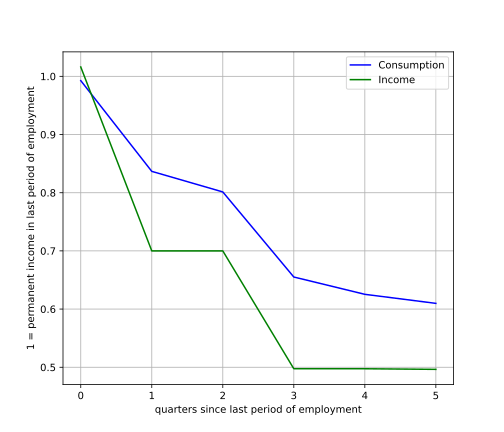
\includegraphics[width=\linewidth]{\econtexRoot/Code/HA-Models/FromPandemicCode/Figures/UnempSpell_Dynamics}
%       \else
%         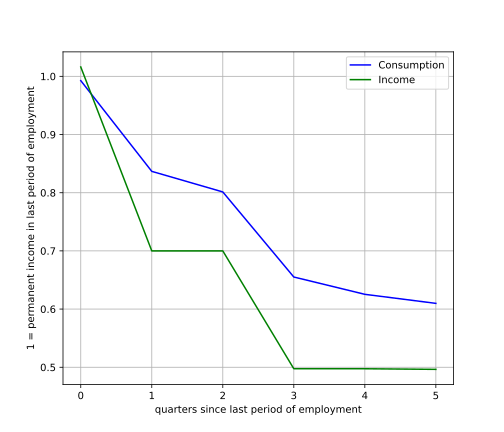
\includegraphics[width=0.48\textwidth]{\econtexRoot/Code/HA-Models/FromPandemicCode/Figures/UnempSpell_Dynamics}
%       \fi
%     }
%     \ifdefined\HCode
%       \HCode{</div>}
%     \fi
%   \end{tabular*}
%   \ifdefined\HCode
%     \HCode{<figcaption style="text-align: center; width: auto; max-width: 800px;">}
%   \fi
%   \caption{Untargeted moments}
%   \notinsubfile{\label{fig:untargetedMoments}}
%   \ifdefined\HCode
%     \HCode{<div style="text-align: justify; width: 16cm; margin: 1em auto 0 auto;">}
%   \fi
%   \parbox{16cm}{\small \vspace{.15cm} \textbf{Note}: Panel (a) compares the dynamic consumption response in the model to the estimates in \citet{fagereng_mpc_2021}; see their Figure~A5. Panel (b) shows the evolution of income and spending for households who remain unemployed long enough for UI benefits to expire; see Figure~2 in \citet{ganongConsumer2019}.\normalsize}
%   \ifdefined\HCode
%     \HCode{</div>}
%   \fi
%   \ifdefined\HCode
%     \HCode{</figcaption></div>}
%   \fi
% \end{figure}

\ifthenelse{\boolean{Web}}{}{
  \end{document} \endinput
}


\newcommand{\econtexRoot}{.}

\documentclass[\econtexRoot/HAFiscal]{subfiles}
\onlyinsubfile{\externaldocument{\econtexRoot/HAFiscal}} % Get xrefs -- esp to apndx -- from main file; only works if main file has already been compiled

\begin{document}
	
\FloatBarrier
\hypertarget{hank}{}\par\section{Robustness in a HANK and SAM Model}
\notinsubfile{\label{sec:hank}}


The main results of this paper are presented in a partial equilibrium setup with aggregate demand effects that do not arise from general equilibrium effects. We think there are many advantages to studying the welfare and multiplier effects in this setting without embedding the model in general equilibrium.  First, general equilibrium models often struggle to adequately capture the feedback mechanisms between consumption and income, particularly the asymmetric nature of these relationships during recessionary versus expansionary periods. Additionally, a complete general equilibrium treatment would necessitate the analysis of numerous complex channels including investment dynamics, firm ownership structures and dividend distribution policies, inventory management, and international trade flows—elements that, while important in their own right, would potentially obscure the core mechanisms we aim to investigate.

Despite the advantages of our partial equilibrium approach, here we complement our analysis with a general equilibrium HANK and SAM model, as standard as possible, that is able to capture supply-side effects that are absent from the partial equilibrium model. In particular, fiscal policies can generate labor market responses that our partial equilibrium analysis does not address. These supply-side channels can affect both the welfare implications and the fiscal multipliers of different policy interventions. Furthermore, standard to the HANK and SAM literature, the general equilibrium model generates a self-reinforcing precautionary saving channel that amplifies business cycles. During a recession, heightened unemployment risk prompts households to increase savings and reduce consumption which in turn weakens both aggregate and labor demand. The resulting decline in labor demand further raises unemployment risk, reinforcing precautionary savings.

We embed the consumption choices of our households—--with heterogeneity over education type and discount factors—--in a New Keynesian model with search and matching frictions that closely follows \cite{Du2024}, which, in turn, is in spirit of the seminal work of \cite{Ravn2017,Ravn2021}. Aside from the consumption block of the model, the framework is standard and follows from the HANK and SAM literature. The model features nominal price rigidities \`{a} la Rotemberg, a monetary authority that sets the nominal interest rate following a standard Taylor rule that responds to inflation, and a fiscal authority that taxes labor income and borrows debt from households to fund unemployment insurance and interest on past debt. As in \cite{Gornemann2021}, \cite{Bardoczy2022}, and \cite{gravesUnemployment}, households randomly search for jobs and match with a labor agency that sells labor to intermediate good producers. Complete details of the model are provided in appendix \ref{sec:hank_appendix}. 

The general equilibrium structure generates fiscal multipliers through an intertemporal Keynesian cross mechanism, which becomes particularly pronounced when monetary policy is passive. Moreover, the search and matching framework allows the employment rate to respond to policy interventions, allowing us to capture both demand and supply effects of fiscal policies.

Our approach in this section relies on linearizing the macro dynamics of the model and employs the Sequence Space Jacobian methods developed by \cite{Auclert2021}. This linearization imposes certain constraints on our analysis. Notably, we cannot evaluate the effects of different policies starting from a deep recessionary state, as we do in our main results.\footnote{One approach to overcome this limitation, which could be used in future work, is described in \cite{bmpMITshocks}.} This limitation prevents us from conducting welfare comparisons between recessionary periods and the steady state. Additionally, the Keynesian cross mechanism embedded in the model exhibits uniform behavior regardless of the degree of economic slack—--a feature that stands in contrast to the state-dependent multipliers we apply in our partial equilibrium analysis.\footnote{We note two additional technical limitations of our general equilibrium implementation. First, stimulus payments in the model are specified as proportional to permanent income, rather than as means-tested fixed dollar amounts as implemented in practice and in our partial equilibrium framework. Second, splurge behavior only occurs out of equilibrium.} 



The consumption response in this general equilibrium model to each of the three policies is shown in the top row of Figure~\ref{fig:HANK_IRFs}. For each of the three fiscal policies, we have shown the consumption response under three different monetary policy rules: 1) an active Taylor rule with a coefficient of 1.5 on inflation; 2) a fixed nominal rate (simulating an effective lower bound); and 3) a fixed real rate (closest in spirit to our partial equilibrium analysis).

%Old figure with just the impulse response
\begin{comment}
\begin{figure}[th]
	\begin{center}
		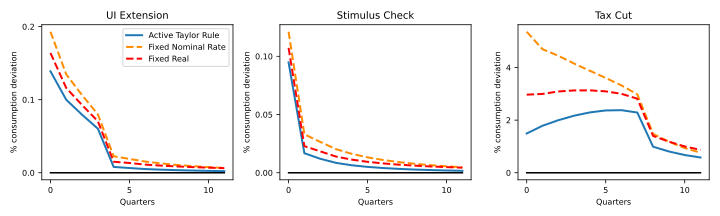
\includegraphics[width=.9\textwidth]{../Figures/HANK_IRFs_w_splurge}
		\caption{Consumption Impulse Responses to Each Policy in the HANK and SAM Model}
		\notinsubfile{\label{fig:HANK_IRFs}}
	\end{center}
\end{figure}
\end{comment}


\begin{figure}[htb]
	\centering
	\begin{subfigure}[b]{.33\linewidth}
		\centering
		\includegraphics[width=\linewidth]{\econtexRoot/Code/HA-Models/FromPandemicCode/Figures/HANK_transfer_irf}
		\caption{stimulus check - IRF}
		\notinsubfile{\label{fig:hank_stimulus_irf}}
	\end{subfigure}%
	\begin{subfigure}[b]{.33\linewidth}
		\centering
		\includegraphics[width=\linewidth]{Code/HA-Models/FromPandemicCode/Figures/HANK_UI_irf}
		\caption{UI extension - IRF}
		\notinsubfile{\label{fig:hank_UI_irf}}
	\end{subfigure}%
	\begin{subfigure}[b]{.33\linewidth}
		\centering
		\includegraphics[width=\linewidth]{Code/HA-Models/FromPandemicCode/Figures/HANK_tax_irf}
		\caption{payroll tax cut - IRF}
		\notinsubfile{\label{fig:hank_tax_irf}}
	\end{subfigure}\\
	\begin{subfigure}[b]{.33\linewidth}
		\centering
		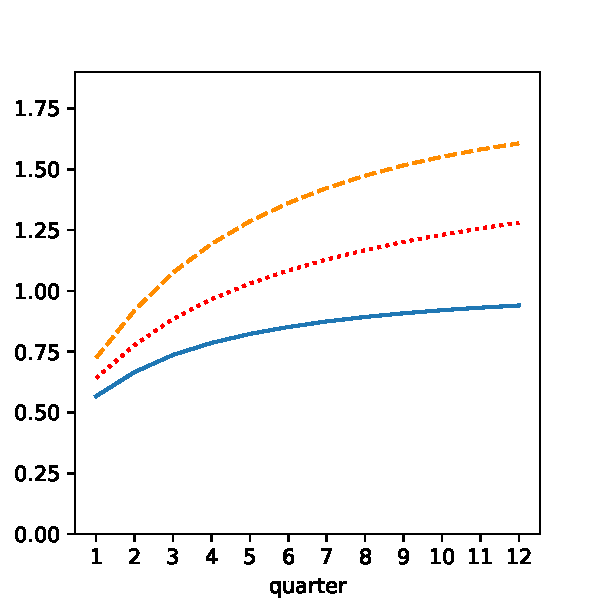
\includegraphics[width=\linewidth]{\econtexRoot/Code/HA-Models/FromPandemicCode/Figures/HANK_transfer_multiplier}
		\caption{stimulus check - cumulative multiplier}
		\notinsubfile{\label{fig:HANK_transfer_multiplier}}
	\end{subfigure}%
	\begin{subfigure}[b]{.33\linewidth}
		\centering
		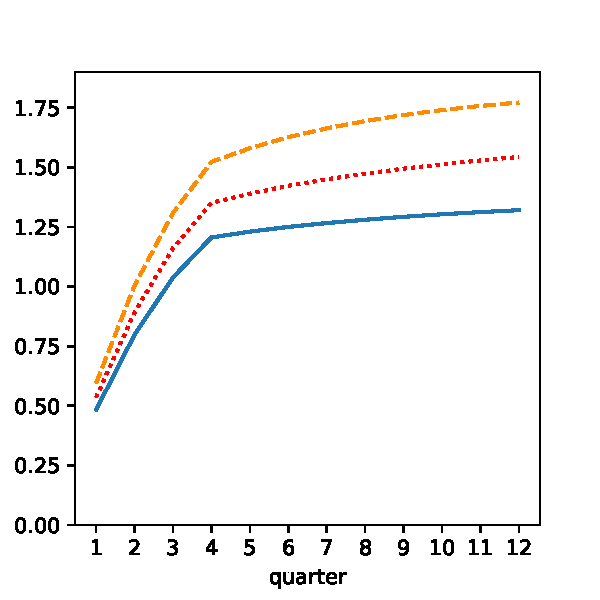
\includegraphics[width=\linewidth]{Code/HA-Models/FromPandemicCode/Figures/HANK_UI_multiplier}
		\caption{UI extension - cumulative multiplier}
		\notinsubfile{\label{fig:HANK_UI_multiplier}}
	\end{subfigure}%
	\begin{subfigure}[b]{.33\linewidth}
		\centering
		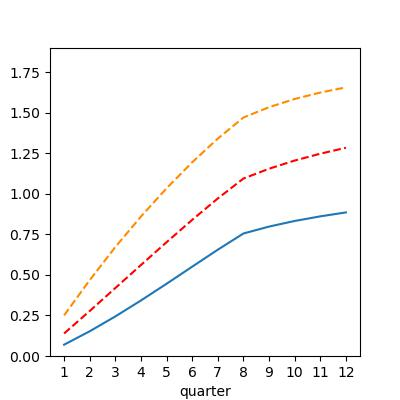
\includegraphics[width=\linewidth]{Code/HA-Models/FromPandemicCode/Figures/HANK_tax_multiplier}
		\caption{payroll tax cut - cumulative multiplier}
		\notinsubfile{\label{fig:HANK_tax_multiplier}}
	\end{subfigure}
	\caption{Impulse responses of aggregate consumption to policy shocks as well as cumulative multipliers as a function of the horizon for the three policies. {\label{fig:HANK_IRFs}}}
\end{figure}



Overall, the IRFs from this model are similar to those from the partial equilibrium analysis, especially under the fixed real-rate rule. Note that the magnitude of the consumption response to the UI extension is lower than in our main analysis---a consequence of lower long-term unemployment in this HANK exercise of deviating from the steady state.\footnote{By contrast, our main analysis considers deviations from a recessionary scenario. Note that the dynamics of the UI extension IRF are also somewhat faster acting.
This is because, under the recession that we study in the partial equilibrium analysis, the large mass of newly-unemployed households do not start receiving extended UI for six months.
} Furthermore, although we are unable to repeat our welfare analysis under a recession in this model, the distributional effects of the policies are similar.
Most importantly, the mechanism leading to far greater welfare benefits for the UI extension, namely that the newly unemployed have high marginal utility, are robust to the supply-side effects of a general equilibrium HANK and SAM model.

\begin{figure}[th]
	\begin{center}
		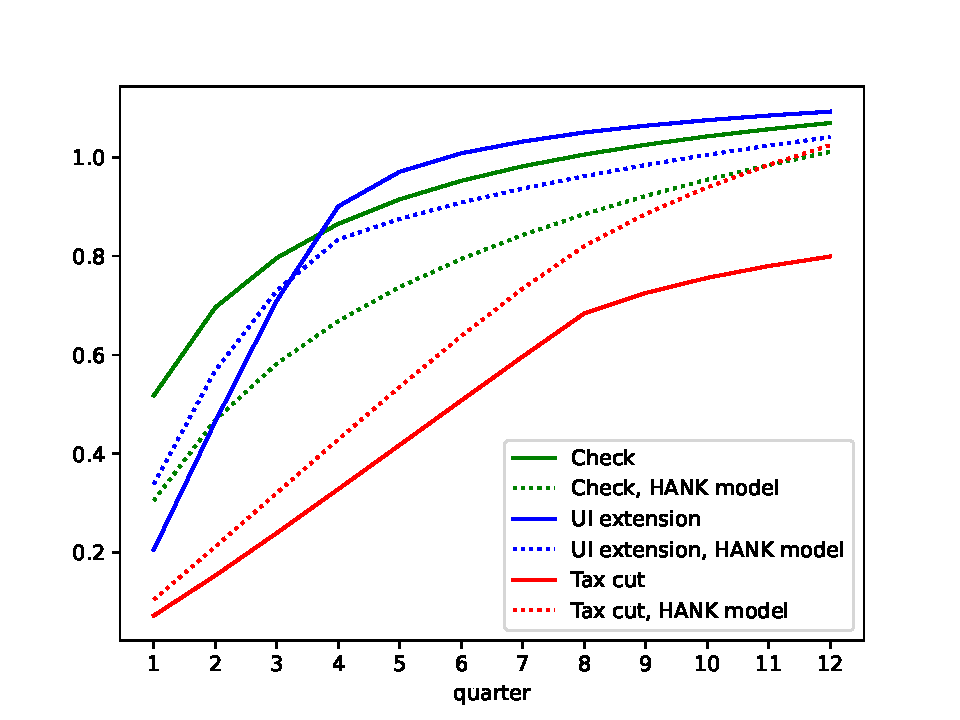
\includegraphics[width=.9\textwidth]{\econtexRoot/Code/HA-Models/FromPandemicCode/Figures/Cummulative_multipliers_withHank}
		\caption{Consumption multiplier as a function of the horizon for the three policies in the partial equilibrium vs the HANK model}
		\parbox{16cm}{\small \vspace{.15cm} \textbf{Note}: In the partial equilibrium model, policies are implemented during a recession with aggregate demand effect active.\normalsize}
		\notinsubfile{\label{fig:HANK_multipliers}}
	\end{center}
\end{figure}


The bottom row of Figure~\ref{fig:HANK_IRFs} shows the corresponding cumulative multipliers for each policy and monetary policy rule. Figure \ref{fig:HANK_multipliers} compares these consumption multipliers over different horizons under a fixed real rate rule to those in our baseline partial equilibrium model.
The multipliers are bigger in the HANK and SAM model.
Nevertheless, in both models, the relative ranking of the consumption multipliers over time horizons are similar, with the effect of the tax cut substantially smaller than the stimulus check or UI extension policies, despite the inclusion of supply-side effects in this HANK model.
However, in contrast to the partial equilibrium model, towards the end of the period shown the tax cut consumption multiplier is near that of the stimulus check.
This is because the aggregate demand effects in our partial equilibrium model do not continue beyond the recession, dampening the benefits of the tax cut policy---in which much of the extra spending occurs after the recession is over---relative to the stimulus check and extended UI policies.


\ifthenelse{\boolean{Web}}{}{
\end{document} \endinput
}
\newcommand{\econtexRoot}{.}

\documentclass[\econtexRoot/HAFiscal]{subfiles}
\onlyinsubfile{\providecommand{\econtexRoot}}
\onlyinsubfile{\renewcommand{\econtexRoot}{..}}
\onlyinsubfile{\externaldocument{\econtexRoot/HAFiscal}} % Get xrefs -- esp to apndx -- from main file; only works if main file has already been compiled

\begin{document}

\FloatBarrier
\hypertarget{comparing-fiscal-stimulus-policies}{}\par\section{Comparing fiscal stimulus policies}
\notinsubfile{\label{sec:comparing}}

In this section, we present our results where we compare three policies to provide fiscal stimulus in our calibrated model. The policies we compare are a means-tested stimulus check, an extension of unemployment benefits, and a payroll tax cut. Each policy is implemented at the start of a recession, and we compare results both with and without aggregate demand effects being active during the recession. First, we present impulse responses of aggregate income and consumption after the implementation of each policy. Then we compare the policies in terms of their cumulative multipliers and in terms of their effect on a welfare measure that we introduce. Finally, based on these comparisons, we can rank the three policies. 

\hypertarget{impulse-responses}{}\par\subsection{Impulse responses}
\notinsubfile{\label{sec:IRFs}}

The impulse responses that we present for each stimulus policy are constructed as follows: 
\begin{itemize} 
\item A recession hits in quarter one. 
\item We compute the subsequent path for the economy without any policy introduced in response to the recession. 
\item We also compute the subsequent path for the economy with a given policy introduced at the onset of the recession in quarter one. 
\item The impulse responses we present are then the \textit{difference} between these two paths for the economy and show the effect of a policy relative to a case where no policy was implemented.
\item The solid lines show these impulse responses for an economy where the aggregate demand effects described in section~\ref{sec:ADeffects} are not active, and the dashed lines show impulse responses for an economy where the aggregate demand effects are active during the recession. 
\item Red lines refer to aggregate labor and transfer income, and blue lines refer to consumption. 
\end{itemize}

Note that all graphs show the average response of income and consumption for recessions of different length.
Specifically, we simulate recessions lasting from only one quarter up to 20 quarters.
We then take the sum of the results across all recession lengths weighted by the probability of this recession length occurring (given our assumption of an average recession length of six quarters).

\subsubsection{Stimulus check} 



\begin{figure}[htb]
	\centering
	\begin{subfigure}[b]{.33\linewidth}
		\centering
		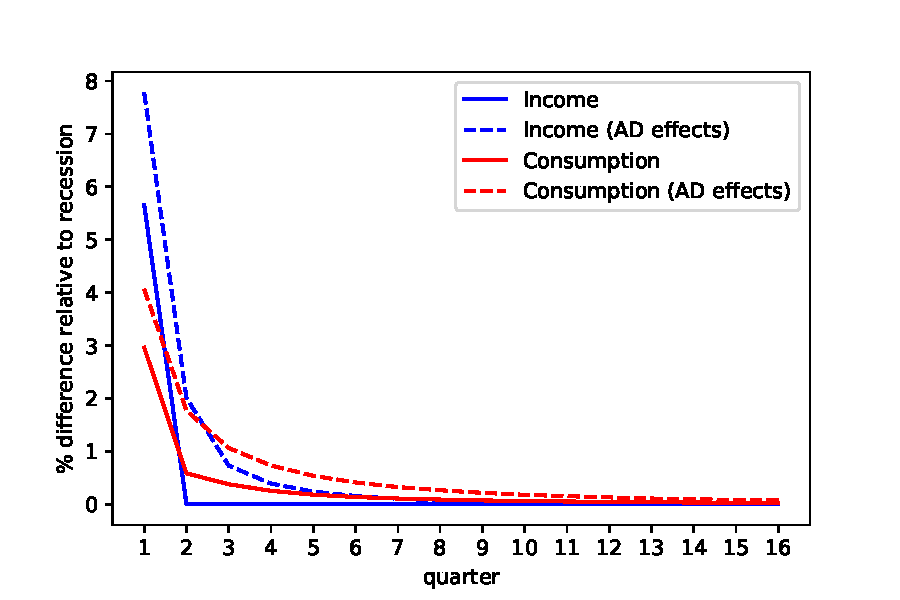
\includegraphics[width=\linewidth]{\econtexRoot/Code/HA-Models/FromPandemicCode/Figures/recession_Check_relrecession}
		\caption{stimulus check - IRF}
		\notinsubfile{\label{fig:recessioncheckrelrecession}}
	\end{subfigure}%
	\begin{subfigure}[b]{.33\linewidth}
		\centering
		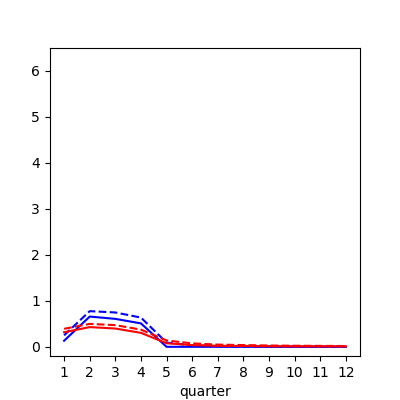
\includegraphics[width=\linewidth]{Code/HA-Models/FromPandemicCode/Figures/recession_UI_relrecession}
		\caption{UI extension - IRF}
		\notinsubfile{\label{fig:recessionuirelrecession}}
	\end{subfigure}%
	\begin{subfigure}[b]{.33\linewidth}
		\centering
		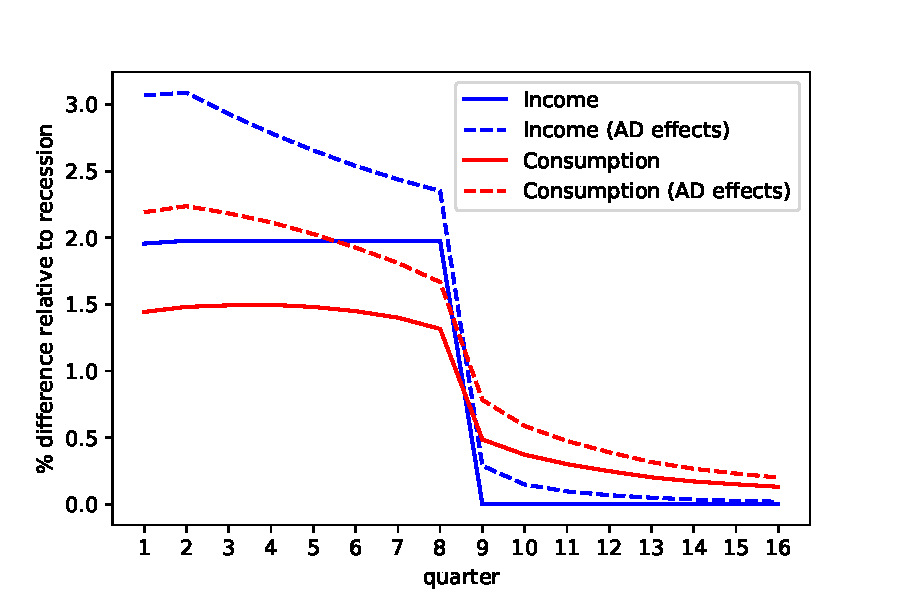
\includegraphics[width=\linewidth]{Code/HA-Models/FromPandemicCode/Figures/recession_taxcut_relrecession}
		\caption{payroll tax cut - IRF}
		\notinsubfile{\label{fig:recessiontaxcutrelrecession}}
	\end{subfigure}\\
		\begin{subfigure}[b]{.33\linewidth}
		\centering
		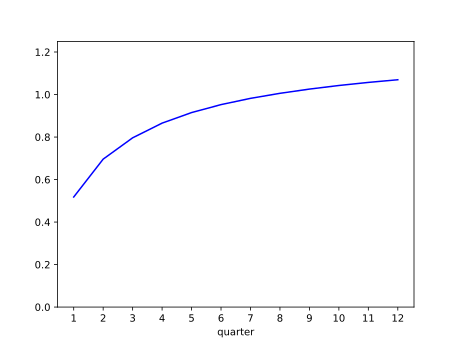
\includegraphics[width=\linewidth]{\econtexRoot/Code/HA-Models/FromPandemicCode/Figures/Cummulative_multiplier_Check}
		\caption{stimulus check - cumulative multiplier}
		\notinsubfile{\label{fig:recessioncheckrelrecession_Mult}}
	\end{subfigure}%
	\begin{subfigure}[b]{.33\linewidth}
		\centering
		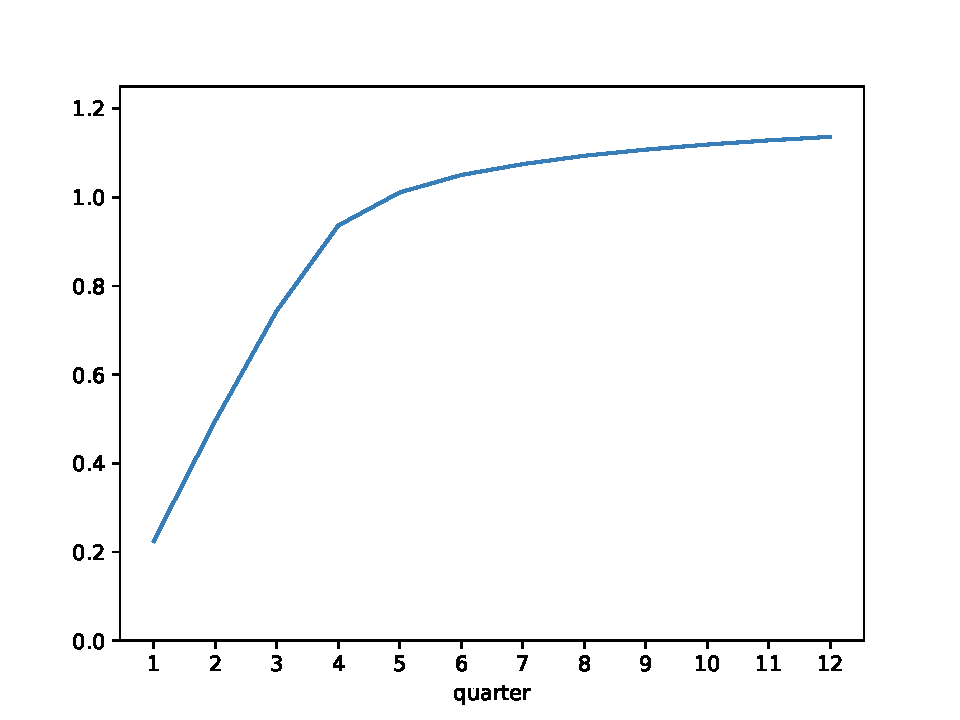
\includegraphics[width=\linewidth]{Code/HA-Models/FromPandemicCode/Figures/Cummulative_multiplier_UI}
		\caption{UI extension - cumulative multiplier}
		\notinsubfile{\label{fig:recessionuirelrecession_Mult}}
	\end{subfigure}%
	\begin{subfigure}[b]{.33\linewidth}
		\centering
		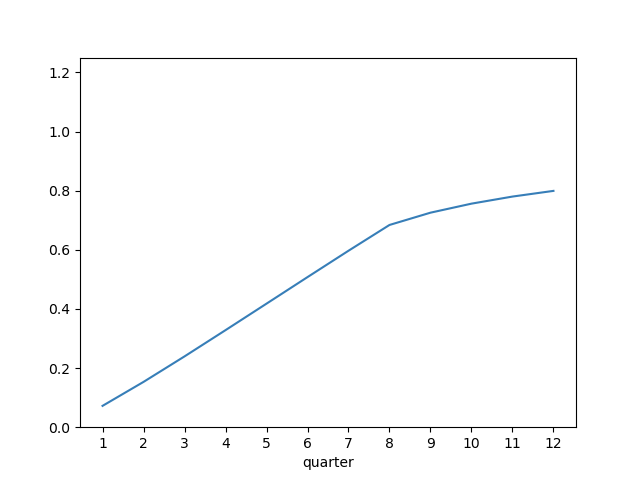
\includegraphics[width=\linewidth]{Code/HA-Models/FromPandemicCode/Figures/Cummulative_multiplier_TaxCut}
		\caption{payroll tax cut - cumulative multiplier}
		\notinsubfile{\label{fig:recessiontaxcutrelrecession_Mult}}
	\end{subfigure}
	\caption{Impulse responses of aggregate income and consumption to policy shocks during recessions with and without aggregate demand effects as well as cumulative multipliers as a function of the horizon for the three policies. {\label{fig:Policyrelrecession}}}
	\parbox{16cm}{\small \vspace{.15cm} \textbf{Note}: For the cumulative multiplier plots, policies are implemented during a recession with aggregate demand effects active.\normalsize}
\end{figure}



Figure \ref{fig:recessioncheckrelrecession} shows the impulse response of income and consumption when stimulus checks are issued in the first quarter of a recession.
In the model without a multiplier, the stimulus checks account for 5 percent of the first quarter's income.
In the following quarters, there are no further stimulus payments, and income remains the same as it would have been without the stimulus check policy.
Consumption is about 2.5 percent higher in the first quarter, which includes the splurge response to the stimulus check.
Consumption then drops to less than 1 percent above the counterfactual, and the remainder of the stimulus check money is then spent over the next few years.
In the model with aggregate demand effects, income in the first quarter is 6 percent higher than the counterfactual, as the extra spending feeds into higher incomes.
Consumption in this model jumps to a higher level than without aggregate demand effects and comes down more slowly as the feedback effects from consumption to income dampen the speed with which income---and hence the splurge---return to zero.
After a couple of years, when the recession is most likely over and aggregate demand effects are no longer in place, income is close to where it would be without the stimulus check policy, although consumption remains somewhat elevated.

\subsubsection{UI extension}


The impulse responses in figure \ref{fig:recessionuirelrecession} show the response to a policy that extends unemployment benefits from 6 months to 12 months for a period of a year.
In the model without aggregate demand effects, the path for income now depends on the number of consumers who receive the extended unemployment benefits.
These consumers are those who have been unemployed for between 6 and 12 months.
In the first quarter of the recession, the newly unemployed receive unemployment benefits regardless of whether they are extended or not.
Therefore, it is in the second and third quarters, when the effects of the recession on long-term unemployment start to materialize, that the extended UI payments ramp up, amounting to an aggregate increase in quarterly income by 0.7 percent.
By the fifth quarter, the policy is no longer in effect, and income from extended unemployment goes to zero.
Consumption in the first quarter jumps by more than income (by 0.3 percent), prompted by both the increase in expected income and the reduced need for precautionary saving given the extended insurance.
In the model without aggregate demand effects, consumption is only a little above the counterfactual by the time the policy is over.
In the model with aggregate demand effects, there is an extra boost to income of about the same size in the first and second quarters.
As this extra aggregate demand induced income goes to employed consumers, more of it is saved, and consumption remains elevated several quarters beyond the end of the policy.

\subsubsection{Payroll tax cut}



The final impulse response graph, figure \ref{fig:recessiontaxcutrelrecession}, shows the impulse response for a payroll tax cut that persists for two years (eight quarters).
In the model without aggregate demand effects, income rises by close to 2 percent as the take-home pay for employed consumers goes up.
After the two-year period, income drops back to where it would have been without the payroll tax cut.
Consumption jumps close to 1 percent in response to the tax cut.
Over the period in which the tax cut is in effect, consumption rises somewhat as the stock of precautionary savings goes up.
Following the drop in income, consumption drops sharply because of the splurge and then decreases over time as consumers spend out the savings they built up over the period the tax cut was in effect.
In the model with aggregate demand effects, income rises by about 2.3 percent above the counterfactual and then declines steadily as the probability that the recession remains active---and hence the aggregate demand effects in place---goes down over time.
Following the end of the policy, the savings stock in the model with aggregate demand effects is high, and consumption remains significantly elevated through the period shown.

\hypertarget{multipliers}{}\par\subsection{Multipliers}
\notinsubfile{\label{sec:multipliers}}

In this section, we compare the fiscal multipliers across the three stimulus policies.
Specifically, we employ the cumulative multiplier, which captures the ratio between the net present value (NPV) of stimulated consumption up to horizon $t$ and the full-horizon NPV of the cost of the policy.
We thus define the cumulative multiplier up to horizon $t$ as
\begin{equation}
	\label{eqn:cumMultiplier}
  M(t) = \frac{NPV(t,\Delta C)}{NPV (\infty,\Delta G)},
\end{equation}
where $\Delta C$ is the additional aggregate consumption spending up to time $t$ in the policy scenario relative to the baseline and $\Delta G$ is the total government expenditure caused by the policy.
The NPV of a variable $X_t$ is given by 
$NPV(t,X) = \sum_{s=0}^{t} \left( \prod_{i=1}^{s} \frac{1}{R_i} \right) X_s$.

The multiplier hence captures the amount of induced consumption at different horizons relative to the total (i.e.
full-horizon) cost of the policies.\footnote{In the case that there is no aggregate demand effect, these multipliers converge to 1 as $t$ goes to infinity.}


The second row in Figure \ref{fig:Policyrelrecession} plots the cumulative multipliers at different horizons, and table \ref{tab:Multiplier} shows the 10y-horizon multiplier for each policy.
The stimulus check, which is paid out in quarter one, exhibits the largest multiplier on impact.
About 50 percent of the total policy expenditure is immediately spent by consumers.
After two years, and because of the aggregate demand effects, consumption has increased cumulatively by more than the cost of the stimulus check.
Over time, the policy reaches a total multiplier of 1.199.
Without AD effects the policy only generates a multiplier of 0.854.
The last two rows in table \ref{tab:Multiplier} show the expected share of the policy expenditures and stimulated consumption that occurs during a recession.
For the stimulus check all of the policy expenditures occur in the first quarter and thus with certainty during the recession.
However, since induced consumption also takes place during later periods at which time the recession may have already ended, the share of stimulated consumption during the recession is lower at 75\%.

Since spending for the UI policy is spread out over four quarters (and peaks in quarters two to three), the multiplier in the first quarter is considerably lower than in the case of the stimulus check.
However, the UI extension policy is targeted in the sense that it provides additional income to only those consumers, who, because of unemployment, have large MPCs.
Also, over the medium-term UI extension expenditures are more likely to induce consumption spending during the recession compared to the check stimulus, see the last row in table \ref{tab:Multiplier}.
This is because UI extension expenditures affect agents who spent the additional income relatively quickly once it reaches them.
Therefore, the cumulative mulitiplier of the UI extension exceeds that of the stimulus check after about one year.


\begin{table}[t]
  \center
  \begin{tabular}{@{}lccc@{}} 
\toprule 
& Tax Cut    & UI extension    & Stimulus check    \\  \midrule 
Long-run Multiplier (AD effect) &1.084  & 1.280  & 1.347     \\ 
Long-run Multiplier (1st round AD effect only) &0.000  & 0.000  & 0.000     \\ 
Share of policy expenditure during recession &57.6\%  & 80.6\%  & 100.0 \%    \\ 
\end{tabular}  

  \caption{Multipliers as well as the share of the policy expenditure and consumption stimulus occurring during the recession}
  \parbox{16cm}{\small \vspace{.15cm} \textbf{Note}: Policies are implemented during a recession with or without the aggregate demand effect active. The row "1st round AD effect only" captures the direct consumption impact of the policies and the additional boost to consumption resulting from the aggregate demand effect acting on the direct consumption impact. It does not include higher-round aggregate demand effects materializing on aggregate demand effects acting on indirectly stimulated consumption.\normalsize}
  \notinsubfile{\label{tab:Multiplier}}
\end{table}

The payroll tax cut has the lowest multiplier irrespective of the considered horizon.
A multiplier of close to 1 is reached only after 10 years with AD effects.
These relatively small numbers reflect that policy spending lasts for a long time and is thus more likely to occur after the recession has ended.
Moreover, only employed consumers, often with relatively low MPCs, benefit directly from the payroll tax cut.
Therefore, the policy is poorly targeted if the goal is to provide short-term stimulus.

Table \ref{tab:Multiplier} contains an additional (middle) row with results for an economy where we only consider a ``first-round'' aggregate demand effect.
To understand these values note that the policies initially increase the income of consumers directly, which leads to a boost in consumption.
As a consequence, this boost triggers an aggregate demand effect which increases the income of everyone and in turn leads to an additional boost to consumption.
We refer to the sum of this initial and the indirect boost to consumption as the first-round AD effect.
However, the AD effect continues as the indirect boost to consumption triggers another round of income increases which further boost consumption and so on.
One might argue that these higher-order rounds of the AD effect are not likely to be anticipated by consumers.
Since higher-order consumption boosts only materialize if consumers anticipate them and act accordingly, the overall increase in consumption might turn out to be smaller than suggested by the full AD effect.
As shown in the middle row of the table, the multipliers are smaller when excluding higher-order rounds.
Nevertheless, the ranking of the policies remains unchanged.


\hypertarget{welfare}{}\par\subsection{Welfare}
\notinsubfile{\label{sec:welfare}}

In this section, we look at the welfare implications of each stimulus policy.
To do so, we need a way to aggregate welfare in our model with individual utility functions.
In our model, some households consume much less than other households, and a social planner with equal weights on each household could significantly increase welfare through redistribution across households even in normal times.
We are interested in the benefit of carrying out fiscal policies in a recession, so we do not want our results to reflect the benefits of redistribution inherent in our model in normal times.

Our welfare measure weights the felicity of a household at time $t$ by the inverse of the marginal utility of the same household in a counterfactual simulation in which neither the recession occurred nor the fiscal policy was implemented, discounted by the real interest rate.\footnote{Discounting at the real interest rate accounts for the fact that a redistributive policy over time will require borrowing or lending at the real interest rate.
The preference discount factors of households would appear in both the numerator and the denominator---the utility and marginal utility---and therefore cancel and do not play a role in our welfare measure.} This weighting scheme means that in normal times the marginal benefit or cost to a social planner of moving a dollar of consumption from one household at one time period to another household at the same or a different time period is zero.
Hence, in normal times, any re-distributive policy has zero marginal benefit.
However, in a recession when the average marginal utility is higher than in normal times, there can be welfare benefits to government borrowing to allow households to consume more during the recession.

As with all social welfare measures, ours is not without ethical issues.  We have chosen our welfare measure over one with equal weights because an equal-weights measure would be increasing with the size of any redistributive policy.\footnote{Using a version of an equal-weights measure results in an even greater welfare benefit to extended unemployment insurance---see the previously distributed draft of this paper, \cite{carroll2023welfare}.  However, because the size of the extended unemployment benefits policy is much larger in a recession compared to normal times, while the size of the other two policies does not change significantly in a recession, this equal-weights measure almost mechanically favored the extended unemployment benefits policy.}  However, similar to Negishi weights, our welfare measure gives greater weight to households that are well off.\footnote{Negishi weights have been used in the climate literature as a way to separate the welfare benefits of climate mitigation policies from broader questions about global income redistribution. Our problem of separating the welfare benefits of recession mitigation policies from income redistribution in normal times is similar, but complicated by our incomplete markets setup. With complete markets, under which there is no potential benefit to redistributing consumption across time for any individual household, our measure is identical to Negishi weights.}  Furthermore, our welfare measure distinguishes between households that would have suffered unemployment in normal times and households that are made unemployed as a result of the recession—--giving the latter a higher weight in the social welfare function.

Let $\mathbf{c}_{it,\textit{normal}}$ be the consumption---inclusive of the splurge---of household $i$ at time $t$ in the baseline simulation with no recession and no fiscal policy.
The (undiscounted) marginal utility of an extra unit of consumption for this household in this time period is $ u'(\mathbf{c}_{it,\textit{normal}})$.


Let $\mathbf{c}_{it,\textit{policy},Rec,AD}$ be the consumption of the same household under the fiscal policy, $\textit{policy}$, possibly a recession, $Rec \in \{0,1\}$, and in an economy with or without aggregate demand effects, $AD \in \{0,1\}$.\footnote{In the simulations, household $i$ experiences the same permanent and transitory shock sequence, but in the recession simulation some households experience unemployment during periods in which the same household is employed in the baseline simulation.}

We also denote the net present value of the government expenditures of the policy as $NPV(\textit{policy},Rec,AD)$.
With this notation, we can now define the welfare bang for the buck of a policy as:

\begin{equation}\begin{gathered}\begin{aligned} \label{welfare_def6}
	\mathcal{W}(\text{policy},Rec,AD) =\frac{1}{NPV(\text{policy},Rec,AD)}\sum_{i=1}^{N} \sum_{t=0}^{\infty} \frac{1}{R^t} \frac{u(\mathbf{c}_{it,\textit{policy},Rec,AD}) - u(\mathbf{c}_{it,\textit{none},Rec,AD})}{ u'(\mathbf{c}_{it,\textit{normal}})} ,
\end{aligned}\end{gathered}\end{equation}
% We can consider displaying the equation below instead which looks slightly nicer?
%\begin{equation}\begin{gathered}\begin{aligned} \label{welfare_def6_alt}
%	\mathcal{W}(\text{policy},Rec,AD) =\frac{\sum_{i=1}^{N} \sum_{t=0}^{\infty} \frac{1}{R^t} \frac{u(\mathbf{c}_{it,\textit{policy},Rec,AD}) - u(\mathbf{c}_{it,\textit{none},Rec,AD})}{ u'(\mathbf{c}_{it,\textit{normal}})}}{NPV(\text{policy},Rec,AD)},
%\end{aligned}\end{gathered}\end{equation}

In normal times, this welfare measure will be exactly equal to one for any small-scale fiscal expansion.
To see this, note that the numerator,  $u(\mathbf{c}_{it,\textit{policy},0,0}) - u(\mathbf{c}_{it,\textit{none},0,0})$, is equal to the change in consumption multiplied by the marginal utility in normal times.
As the total change in consumption is equal to the net present value of the policy, which we divide by, the total welfare measure is equal to one.
Note that for large increases in consumption, this measure may be less than one because the utility function is concave.

\begin{table}[ht] 
	\center
	\begin{tabular}{@{}lccc@{}} 
\toprule 
                          & Stimulus check      & UI extension    & Tax cut    \\  \midrule 
$\mathcal{W}(\text{policy}, Rec=0, AD=0)$ & 1.00  & 0.85  & 1.00     \\ 
$\mathcal{W}(\text{policy}, Rec=1, AD=0)$ & 1.03  & 1.83  & 0.98     \\ 
$\mathcal{W}(\text{policy}, Rec=1, AD=1)$ & 1.40  & 2.15  & 1.12     \\ \bottomrule 
\end{tabular}  

	\caption{Welfare measures, calculated for policies implemented both out of and in a recession with and without aggregate demand effects}
	\notinsubfile{\label{welfare6}}
\end{table}

Table \ref{welfare6} shows the welfare measure for each policy as defined by equation \eqref{welfare_def6}.
The top row of the table shows the welfare measure for implementing each policy in normal times.
For marginal policies, this is equal to one by definition.
Indeed, the value for both the stimulus check and the tax cut policy is very close to one.
However, the welfare measure for the extended unemployment policy in normal times is noticeably less than one.
This is because, although this policy is smaller in absolute size than the other policies, its consumption effects are concentrated on a small number of households that remain unemployed long enough to receive the extended benefits.
For these households, the effect on consumption is large enough such that the non linearity of the consumption function leads to smaller welfare benefit than the marginal utility of consumption would otherwise imply.

The second row of table \ref{welfare6} shows the welfare benefit of each policy in a recession without any aggregate demand effects.
Again, the stimulus check and tax cut policies have measures that are close to one---pulling forward consumption has little welfare benefit for the average household because the average marginal utility of consumption is only a little higher than in normal times.
By contrast, the policy sees benefits of 1.8 dollars for every dollar spent on extended UI benefits during a recession.
This is because many of the households who are unemployed for many quarters in the recession would have never been unemployed, or quickly reemployed, in normal times and hence their marginal utility of consumption is much higher in the recession than in normal times.

The third row of the table shows the welfare measure for each policy in a recession in the version of the model with aggregate demand effects during the recession.
The payroll tax cut now has a noticeable benefit, as some of the tax cut gets spent during the recession, resulting in higher incomes for all consumers.
However, the tax cut is received over a period of two years, and much of the relief may be after the recession---and hence the aggregate demand effect---is over.
Furthermore, because the payroll tax cut goes only to employed consumers who have relatively lower MPCs, the spending out of this stimulus will be further delayed, possibly beyond the period of the recession.
By contrast, the stimulus check is received in the first period of the recession and goes to both employed and unemployed consumers.
The earlier arrival and higher MPCs of the stimulus check recipients mean more of the stimulus is spent during the recession, leading to greater aggregate demand effects, higher income, and higher welfare.
The extended UI arrives, on average, slightly later than the stimulus check.
However, the recipients, who have been unemployed for at least six months, spend the extra benefits relatively quickly, resulting in significant aggregate demand effects during the recession.
In contrast to the payroll tax cut, extended UI has the benefit of automatically reducing if the recession ends early, making fewer consumers eligible for the benefit.


\hypertarget{comparing-the-policies}{}\par\subsection{Comparing the policies} 

The results presented in sections~\ref{sec:multipliers} and~\ref{sec:welfare} indicate that the extension of unemployment benefits is the clear ``bang for the buck'' winner.
The extended UI payments are well targeted to consumers with high MPCs and high marginal utility, giving rise to large multipliers and welfare improvements.
The stimulus checks come in slightly higher when measured by their short-term multiplier effect but are a distant second when measured by their welfare effects.
The stimulus checks have large initial multipliers because the money gets to consumers at the beginning of the recession and therefore induce aggregate demand effects more quickly.
However, the checks are not well targeted to high-MPC consumers, so even though the funds arrive early in the recession, they are spent out more slowly than the extended unemployment benefits.\footnote{Theoretically, stimulus checks could be targeted to the highest-MPC households which, for small-sized policies, would mean households with an MPC of one.
However, data limitations and other practicalities make means-testing stimulus checks by income the extent of targeting in practice.} Furthermore, the average recipient of a stimulus check has a much lower marginal utility than consumers receiving unemployment benefits, so the welfare benefits of this policy are substantially muted relative to UI extensions.

The payroll tax cut policy does poorly by both measures: It has a low overall multiplier and negligible welfare benefits.
The reasons are that the funds are slow to arrive, so the subsequent spending often occurs after the end of the recession, and that the payments are particularly badly targeted---they go only to employed consumers.

While it is clear from the analysis that the extended unemployment benefits should be the first tool to use, a disadvantage of them is that they are limited in their size.
If a larger fiscal stimulus is deemed appropriate, then stimulus checks provide an alternative option that will stimulate spending during the recession even if the welfare benefits are substantially lower than the UI extension.


\FloatBarrier
\hypertarget{Model_without_splurge}{}\par\subsection{Results in a model without the splurge} 

We introduce the splurge in our model with the aim of matching empirical evidence on the dynamics of spending in response to transitory income shocks.
The splurge acts as a stand-in for competing theories for why agents may spend more out of those shocks than suggested by a simple model in which forward-looking agents solely maximize utility.
However, it is natural to consider to what extent the splurge is in fact necessary to match the empirical patterns and the implications for our results ranking the different policies.
To assess this we  reestimate the model without the splurge and recompute all our results regarding the relative effectiveness of the policies in this version of the model.

The details of this exercise are in Appendix~\ref{app:Model_without_splurge}.
There we discuss how the estimation of the Norwegian model in section~\ref{sec:splurge} is affected if we do not include splurge consumption, and the estimation of the discount factor distributions for each education group in the US economy without taking the splurge as given.
The general result is that the we can match the liquid wealth distributions that we target also in models that do not include a splurge.
The models do so by estimating wider distributions of discount factors than we found in section~\ref{sec:splurge} and~\ref{sec:estimBetas}.


Without the splurge the models do struggle to exactly match the dynamics of spending after a temporary income shock, however.
In particular, for the estimation of the Norwegian model, we can compare the model's implications for MPCs for different wealth quartiles to empirical estimates.
Without the splurge, the model leads to an MPC for the top wealth quartile that is far lower than in the data.
In the US model this MPC is also quite low compared to the model with splurge consumption, but for the US we do not have an empirical estimate to compare to.


To evaluate the impact of splurge consumption on our ranking of the policies, we simulate the three fiscal policies in the reestimated model without the splurge.
There are only minor shifts in the multipliers of the policies, but the lower average MPCs reduces multipliers for the check and tax cut policy relative to the model with the splurge.
In contrast, the UI extension becomes slighlty more effective in stimulating consumption as the wider distribution of discount factors implies a larger share of the population that hits the borrowing constraint upon expiry of UI benefits.
Hence, the extension of UI benefits affects agents more strongly in the model without the splurge.

More importantly for the main conclusion of our paper, table \ref{tab:welfare6_SplurgeComp} compares the welfare implications of the policies in the two models.
Generally, the welfare metric varies only marginally across the models.
When aggregate demand effects are active, we see slightly larger differences in the welfare evaluation, with the check policy losing ground against the UI extension.
This is because the welfare impact of the check in the model with the splurge is contingent on the checks being spent quickly due to a high average MPC and thus generating strong aggregate demand effects while the recession is still ongoing.
In the absence of the splurge only liquidity-constrained agents spend the check money quickly, such that recession-induced aggregate demand effects are smaller.


\begin{table}[ht] 
	\center
	\begin{tabular}{@{}lccc@{}} 
\toprule 
                          & Stimulus check      & UI extension    & Tax cut    \\  \midrule 
$\mathcal{W}(\text{policy}, Rec=0, AD=0)$ & 0.97(0.96)  & 0.84(0.85)  & 0.99(0.99)     \\ 
$\mathcal{W}(\text{policy}, Rec=1, AD=0)$ & 1.00(0.99)  & 1.80(1.82)  & 0.97(0.98)     \\ 
$\mathcal{W}(\text{policy}, Rec=1, AD=1)$ & 1.27(1.34)  & 2.12(2.11)  & 1.09(1.10)     \\ 
\end{tabular}  

	\caption{Welfare measure, calculated for policies implemented both out of and in a recession with and without aggregate demand effects.}
	\parbox{16cm}{\small \vspace{.15cm} \textbf{Note}: The values outside of the brackets capture the multipliers in the model without the splurge, while those inside the brackets are mulitipliers with the splurge. \normalsize}
	\notinsubfile{\label{tab:welfare6_SplurgeComp}}
\end{table}

Overall, we can conclude that the ranking of the policies remains unaffected by the splurge.
The splurge is thus helpful in matching available empirical evidence, but does not affect the assessment of the effectiveness of the considered policies.











\ifthenelse{\boolean{Web}}{}{
  \end{document} \endinput
}
\newcommand{\econtexRoot}{.}

\documentclass[\econtexRoot/HAFiscal]{subfiles}
\onlyinsubfile{\externaldocument{\econtexRoot/HAFiscal}} % Get xrefs -- esp to apndx -- from main file; only works if main file has already been compiled

\begin{document}

\hypertarget{conclusion}{}\par\section{Conclusion}
\notinsubfile{\label{sec:conclusion}}

For many years leading up to the Great Recession, a widely held view among macroeconomists was that countercyclical policy should be left to central banks, because fiscal policy responses were unpredictable in their timing, their content, and their effects.  Nevertheless, even during this period, fiscal policy responses to recessions were repeatedly tried, perhaps because the macroeconomists' advice to policymakers, ``don't just do something; stand there''---is not politically tenable.

This paper demonstrates that macroeconomic modeling has finally advanced to the point where we can make reasonably credible assessments of the effects of alternative policies of the kinds that have been tried.  The key developments have been both the advent of national registry datasets that can measure crucial microeconomic phenomena and the creation of tools of heterogeneous agent macroeconomic modeling that can match those micro facts and glean their macroeconomic implications.

We examine three fiscal policy experiments that have actually been implemented in the past: an extension of UI benefits, a stimulus check, and a tax cut on labor income.  Our model suggests that the extension of UI benefits is a clear ``bang for the buck'' winner.  While the stimulus check arrives faster and generates multiplier effects more quickly, it is less well targeted to high-MPC households than an extension of UI benefits. By contrast, the welfare gains of extended UI benefits are significantly greater than those of a stimulus check. The chief drawback of the UI extension is that its size is limited by the fact that a relatively small share of the population is affected by it. In contrast, stimulus checks are easily scalable while exhibiting only slightly less recession-period stimulus (in a typical recession). However, since some of the stimulus checks flow to well-off consumers, such checks do worse than UI extensions when we evaluate welfare consequences. Finally, the payroll tax cut is the least effective in terms of both the multiplier and welfare effect, since it targets only employed consumers and, for a typical recession, more of its payouts are likely to occur after the recessionary period (when multipliers may exist) has ended.

The tools we are using could be reasonably easily modified to evaluate a number of other policies.  For example, in the COVID-driven recession, not only was the duration of UI benefits extended, but those benefits were also supplemented by substantial payments to all UI recipients.  We did not calibrate the model to match this particular policy, but the framework could accommodate such an analysis.

\ifthenelse{\boolean{Web}}{}{
  \end{document} \endinput
}

